\chapter{Recuperación de imágenes basadas en su contenido (CBIR)}\label{ch:CBIR}

En el contexto de las ciencias de información, en el Capítulo 1 de \cite{10.5555/1394399} podemos encontrar una definición genérica para el contexto de las ciencias de computación del término "recuperación de información" que dice que:

\begin{definicion}
La recuperación de información, o \emph{information retrieval (IR)}, consiste en encontrar material de una naturaleza no estructurada que satisface una necesidad de información dentro de grandes colecciones.
\end{definicion}

En particular, nos encontramos trabajando en la recuperación de imágenes que pertenece a la categoría de recuperación de información multimedia. Este, a su vez, se divide en dos tipos de recuperación, las basadas en texto, \emph{text-based image retrieval (TBIR)}, o las basadas en su contenido, \emph{content-based image retrieval (CBIR)}.\\

En \cite{content-based} se dice, en que los sistemas TBIR, los usuarios utilizan palabras clave o descripciones de las imágenes como consulta en una base de datos para recuperar las imágenes que sean relevantes a la palabra clave. Para ello, primeramente las imágenes deben de ser anotados con texto ya sea de forma manual o automática. Esto posee la desventaja de que los algoritmos de anotación automática de imágenes no son factibles para generar textos descriptivos para un amplio espectro de imágenes requiriendo la anotación manual que, a su vez, suele ser subjetiva y dependiente del contexto. Como ventaja, al realizar utilizar únicamente texto para describir la imagen, sus consultas son rápidas ya que la coincidencia de cadenas es un proceso que requiere menos tiempo de cómputo.\\

Por otro lado, la recuperación de imágenes basada en el contenido (CBIR), también conocida como consulta por el contenido de una imagen o \emph{query by image content (QBIC)}, es una técnica automatizada que toma una imagen como consulta y devuelve un conjunto de imágenes similares a esta \cite{content-based}. La imagen consultada es convertida en la representación interna de un vector de características usando la misma rutina de extracción que fue utilizada para crear la base de datos. Se utiliza una medida de similitud para calcular las distancias entre los vectores de características de la imagen consultada y de las imágenes destino en la base de datos de características. Por último, la recuperación se realiza mediante un esquema de indexación que facilita la búsqueda eficiente de la base de datos de imágenes \autoref{fig:content-based-esquema}.\\

\begin{figure}[htpb]
  \centering
  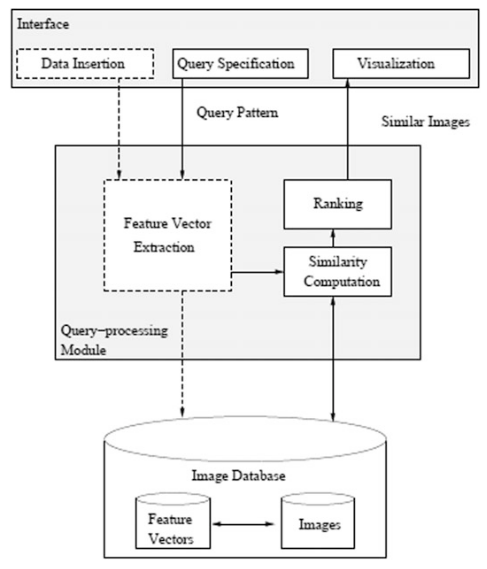
\includegraphics[width=0.55\textwidth]{content-based-esquema}
  \caption{Arquitectura de un sistema CBIR típico. \cite{content-based}}
  \label{fig:content-based-esquema}
\end{figure}

En las páginas 7-8 y 22-26 de \cite{report:39} se mencionan tres niveles de consultas en un CBIR siendo:

\begin{itemize}
\item Nivel 1: La recuperación de imágenes a través de características primitivas como pueden ser diferentes medidas de representación matemática de colores, texturas o formas. Un ejemplo sería un histograma de color que muestra la proporción de píxeles de cada color dentro de la imagen y la consulta sería encontrar imágenes con valores similares.
\item Nivel 2: Comprende la recuperación por características derivadas, también conocidas como lógicas, incluyendo un cierto grado de inferencia lógica sobre la identidad de los objetos representados en la imagen. Además puede ser dividido en:
\begin{itemize}
\item recuperación de objetos de un determinado tipo o categoría. Por ejemplo, ``encuentra imágenes de un autobús de dos pisos''.
\item recuperación de objetos individuales o personas. Por ejemplo, ``encuentra una imagen de la torre Eiffle''.
\end{itemize}
\item Nivel 3: Se trata de la recuperación por atributos abstractos, incluyendo una cantidad significativa de razonamiento de alto nivel sobre el propósito de los objetos o escenas representadas. Por ejemplo, ``encuentra imágenes de una multitud alegre''.
\end{itemize}

El objetivo de este proyecto es desarrollar una aplicación en java que represente un sistema CBIR que siga una arquitectura como la mostrada en \autoref{fig:content-based-esquema}. Este será capaz de extraer distintas características de una imagen y de comparar, o calcular la similitud, entre las imágenes de distintas formas para obtener distintas clasificaciones ordenadas que serán visualizadas en la aplicación. \\

Se podrán realizar consultas de nivel 1 a través de características de color y de nivel 2 utilizando segmentación semántica para la distinción de categorías con una red neuronal implementada en Python.

%\chapter{Planificación y presupuesto.}
\chapter{Requisitos}
Antes de desarrollar la aplicación se debe comenzar con la exposición de los requisitos de datos, funcionales y no funcionales que esta requerirá para así poder tener en mente qué es lo que necesitamos, de qué es lo disponemos y cómo podremos trabajar de forma óptima para llegar al resultado deseado.\\

Teniendo en mente \autoref{fig:content-based-esquema}, sabemos que debemos de tener los siguientes requisitos de datos:\\
\begin{enumerate}
\item Representación de una imagen
\item Vector de características, en adelante descriptor, por cada característica que se quiera extraer o analizar.
\item Base de datos capaz de almacenar los descriptores correspondientes a cada una de las imágenes que estarán almacenadas en dicha base o fácilmente accesibles a través de la información almacenada en ella.
\item Representación de un descriptor genérico almacenado en la base de datos.
\item Concepto de clasificador utilizado para extraer las características.
\item Concepto de comparador para calcular la similitud entre las distintas características.
\end{enumerate}
Seguidamente, respecto a los requisitos funcionales debemos de considerar:\\
\begin{enumerate}
\item Abrir, guardar y cerrar una imagen.
\item Realización de consultas basadas en el contenido de una imagen.
\item Realización de consultas basadas en texto, siendo estas las categorías a las cuales pueden pertenecer nuestras imágenes.
\item Agrupación de categorías.
\item Extracción de descriptores de nivel 1.
\item Extracción de un descriptor de nivel 2.
\item Almacenaje de un conjunto de imágenes para poder ser comparadas.
\item Crear, modificar, guardar y abrir bases de datos.
\item Almacenaje de los descriptores correspondientes a dichas imágenes en una base de datos.
\item Enlace entre las imágenes y sus correspondientes descriptores para un fácil acceso.
\item Comparación entre descriptores.
\item Comparación utilizando múltiples descriptores de las propias imágenes.
\item Ordenación de imágenes resultantes de la consulta utilizando el resultado de la comparación entre descriptores.
\item Capacidad de visualizar las imágenes resultado de forma ordenada según la puntuación obtenida.
\item Capacidad de cambiar los comparadores utilizados sin que se vean afectados los descriptores utilizados.
\item Capacidad de crear nuevas bases de datos utilizando diferentes descriptores.
\item Capacidad de crear nuevas bases de datos utilizando múltiples descriptores.
\item Importar un clasificador a través de un fichero.
\end{enumerate}
Respecto a los requisitos no funcionales nos referimos a las características de funcionamiento que nos servirán para mantener la calidad de nuestro programa. Estos serán, principalmente: rendimiento, durabilidad, estabilidad, seguridad, eficiencia, compatibilidad, garantía e integración de datos. No debemos de olvidarnos tampoco de la necesidad de obtener una gran cantidad de datos para poder entrenar la red neuronal, siendo que en este caso se utiliza el conjunto de datos COCO \cite{COCO}.\\

Finalmente, se debe comentar que todo el proyecto deberá de poder ejecutarse en ordenadores que no dispongan de muchos recursos en unos tiempos razonables, al ser el material del que se dispone y siendo esta la prueba del funcionamiento en uno de los peores casos posibles.

\chapter{Análisis}
Comenzaremos analizando los requisitos mencionados en el capítulo anterior para poder enfrentarnos correctamente al diseño de nuestro sistema.\\

Para los requisitos de datos se considera el encapsular apropiadamente cada uno de estos en una clase propia que sirva como una correcta representación de cada uno de los conceptos. En particular, si consideramos las especificaciones planteadas en los requisitos funcionales, se hace evidente la necesidad de la utilización de herencia para un correcto diseño del software al haber conceptos genéricos que más adelante se dividen teniendo diferentes especificaciones.\\

Además, es necesario desarrollar una aplicación de escritorio que haga mucho más intuitiva la utilización de cada uno de los elementos a implementar. Así, alguien sin conocimientos de programación, pero con interés o una cantidad relativa de estudios en la materia, podría utilizarla cómodamente.\\

Teniendo también en cuenta que sería ideal que la aplicación fuese multiplataforma y la existencia de la \emph{Java Multimedia Retrieval (JMR)} \cite{JMR}, librería desarrollada por Jesús Chamorro Martínez que resuelve de forma genérica gran parte de las funcionalidades solicitadas, se ha decidido utilizar Java como lenguaje de programación.\\

Sin embargo, se debe de tener en cuenta que este proyecto ha sido planteado bajo la premisa de la utilización de aprendizaje profundo. Este será utilizado para la extracción de características de nivel 2, mediante la utilización de una red neuronal convolucionada \autoref{ch:cnn} que realizará una segmentación semántica para obtener diversas categorías así como los píxeles concretos de cada imagen que pertenecerán a cada categoría \cite{ch:fast-attention}.\\

Si bien existen bibliotecas para el aprendizaje profundo en Java, estas no están tan desarrolladas como podrían estarlo en otros lenguajes de programación como Python. Por ello, se utilizará Python 3 para la creación, el entrenamiento y la carga de los modelos que se lleguen a probar a lo largo del proyecto.\\

Esto plantea la cuestión de cómo resolver la comunicación entre los distintos lenguajes, que será resuelta mediante la utilización de una conexión TCP.\\
\chapter{Diseño}

Como se mencionó en el capítulo anterior, la aplicación será diseñada en dos partes conectadas por una conexión TCP. Comenzaremos mencionando las librerías utilizadas para cada una de las partes, prosiguiendo con mostrar una serie de diagramas que mostrarán la estructura interna utilizará nuestra aplicación haciendo uso del material disponible.

\section{Librerías utilizadas}

Comenzaremos mencionando las librerías utilizadas para la creación, entrenamiento y carga de la red neuronal. Principalmente se ha utilizado:
\begin{enumerate}
\item Tensorflow \cite{tensorflow2015-whitepaper}:  se trata de una plataforma de código abierto de extremo a extremo para el aprendizaje automático. Posee una API para diversos lenguajes de programación como son Javascript y Python además de estar disponible tanto para ordenadores como para dispositivos móviles, en este caso bajo su versión Tensorflow Lite. Como extra, permite utilizar varias CPUs o GPUs, con la consecuente posibilidad de aceleración GPU, y ofrece soporte experimental para \emph{Cloud TPUs} en Keras y Google Colab. En particular se utilizará Tensorflow 2.0 que es compatible con Python 3.5 a 3.8.
\item Keras \cite{chollet2015keras} : es una API construida sobre TensorFlow 2.0 que, según su propia página web, ``está diseñada para seres humanos, no para máquinas''. Está optimizada para GPU, CPU y TPU.Fue concebida para actuar como una interfaz en lugar de un framework de machine learning standalone por lo que ofrece un conjunto de abstracciones más intuitivas y de alto nivel, haciendo más sencillo el desarrollo de modelos de aprendizaje profundo.
\item Classification models Zoo - Keras \cite{classification_models}: se trata de un conjunto de clasificadores entrenados en el conjunto de datos ImageNet \cite{imagenet_cvpr09}. De esta forma podremos obtener clasificadores que no están disponibles ni en Keras ni en TensorFlow, en particular ResNet18 \cite{DBLP:journals/corr/HeZRS15}.
\item Imgaug \cite{imgaug} es una biblioteca para el aumento de imágenes en los experimentos de aprendizaje automático. Soporta un gran rango de técnicas de aumento de datos, permite combinarlas fácilmente y ejecutarlas de forma aleatoria en múltiples núcleos CPU.
\end{enumerate}

Para el tratamiento de los datos resultantes de la red neuronal con el fin de adaptarlos para utilizarlos en la aplicación, se ha utilizado el ecosistema basado en Python SciPy, principalmente las librerías:
\begin{enumerate}
\item SciPy \cite{2020SciPy-NMeth} librería fundamental para el cálculo científico.
\item NumPy \cite{2020NumPy-Array} paquete de vectores n-dimensionales.
\item Pandas \cite{reback2020pandas} \cite{mckinney-proc-scipy-2010} estructura de datos y análisis.
\item Matplotlib \cite{Hunter:2007} trazado completo en 2D.
\end{enumerate}
Además, se ha utilizado scikit-image \cite{scikit-image} (o skimage) que es una colección de algoritmos para procesamiento de imágenes y la visión por computador.\\

Como se mencionó en el capítulo anterior, para como esqueleto genérico del sistema CBIR se utilizará la biblioteca \emph{Java Multimedia Retrieval (JMR)} \cite{JMR} sobre la cual desarrollaremos en más detalle los elementos que utilizaremos. En particular, estaremos utilizando una versión actualizada por Miriam Mengíbar Rodríguez para su trabajo de fin de master \cite{TFM}.\\

\begin{figure}[htpb]
  \centering
  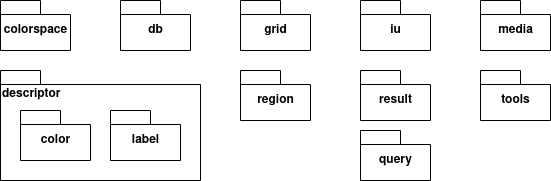
\includegraphics[width=0.9\textwidth]{jmrpackage}
  \caption{Diagrama representante de algunos de los paquetes de la JMR. \cite{JMR}}
  \label{fig:jmrpackage}
\end{figure}

De los paquetes mostrados, concretamente se utilizarán:
\begin{itemize}
\item \emph{db} : Paquete que simula una base de datos. Posee su propio elemento creado a partir de los datos de entrada y de los descriptores, compatibles con la comparación con las consultas y con una cómoda recuperación de los datos originales.
\item \emph{descriptor} : Paquete que engloba los elementos necesarios para una correcta representación de un descriptor o vector de características, como es el caso de la interfaz \emph{Comparator} o la interfaz \emph{MediaDescriptor}. Posee dos subpaquetes:
\begin{itemize}
\item \emph{descriptor.color} : Paquete que implementa descriptores de colores de acuerdo al estándar MPEG7 \cite{MPEG7}.
\item \emph{descriptor.label} : Paquete que implementa un descriptor por etiquetas genérico así como definir las interfaces necesarias para la clasificación de las etiquetas.
\end{itemize}
\item \emph{region} : Paquete diseñado para la representación de una región contenida en una imagen. Si bien este paquete no se ha utilizado directamente, servirá como inspiración para la definición de la clase \emph{MultiRegion} que se verá más adelante.
\end{itemize}

Además, también se utilizarán las clases \emph{LabelGroup} y \emph{TCPClient}, siendo esta última a través de la cual se consigue la conexión TCP con el módulo de python, ambas implementas por Miriam en su trabajo de fin de master \cite{TFM}.

\newpage
\section{Descriptores}
A la hora de diseñar los descriptores, debemos de tener especial atención en no diseñar nada de lo que ya dispongamos. Por ello, no será necesario el diseño de descriptores de nivel 1 de tipo color, puesto que estos ya están diseñados e implementados a través de los paquetes \emph{descriptor} y \emph{descriptor.color} de la JMR \cite{JMR}.\\

El principal trabajo será el diseño e implementación de un descriptor de nivel 2 con su respectivo comparador. En particular, se ha diseñado el descriptor \emph{RegionLabelDescriptor} que, dada una imagen, describirá cada una de las categorías pertenecientes a dicha imagen así como los píxeles concretos que pertenecerán a cada una de estas categorías. De esta forma, no sólo conoceremos qué etiquetas o categorías estarán presentes en la propia imagen sino que además la localización a nivel de píxel de cada una de estas categorías.\\

\begin{figure}[htpb]
  \centering
  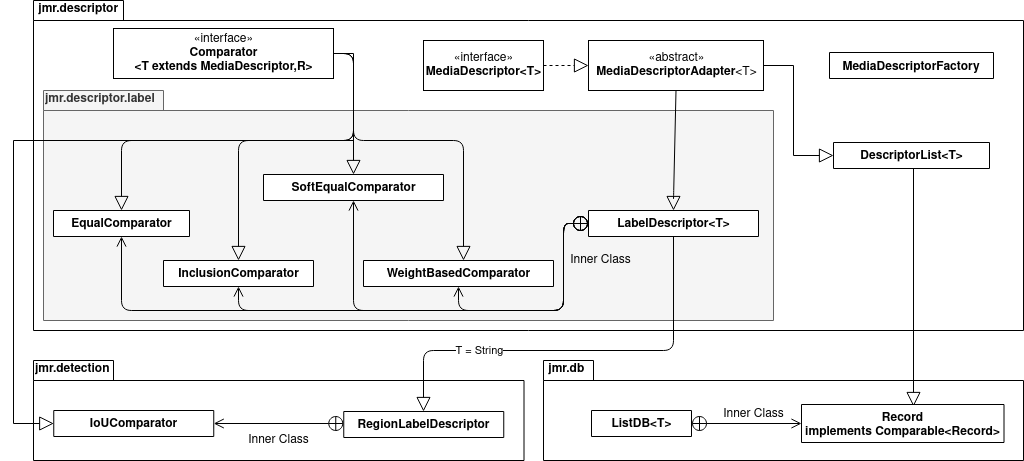
\includegraphics[width=1.1\textwidth]{DescriptorsAndComparators}
  \caption{Diagrama de herencia y clases internas para los descriptores y comparadores de etiquetas. \cite{JMR}}
  \label{fig:DescriptorsAndComparators}
\end{figure}

Para la extracción de estas características para la creación de este descriptor, se ha definido un clasificador llamado \emph{AttentionClassifier} que recibirá la url de la imagen cuyas características se desean extraer y, a través del uso de la clase \emph{TCPClient}, se conectará con un servidor de python llamado \emph{server.py} que segmentará semánticamente la imagen. Con esta información, almacenada en un objeto de la clase \emph{RegionClassification}, se construirá correctamente un objeto \emph{RegionLabelDescriptor} que podrá ser comparado utilizando los comparadores internos de su clase madre \emph{LabelDescriptor} y el comparador \emph{IoUComparator} que se definirá y creará para este descriptor concreto.\\

\begin{figure}[htpb]
  \centering
  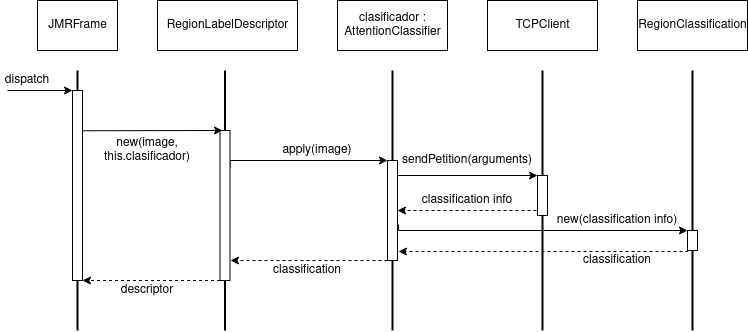
\includegraphics[width=1.1\textwidth]{DiagramaSecuencia}
  \caption{Diagrama de secuencia que muestra la creación de un descriptor del tipo \emph{RegionLabelDescriptor}}
  \label{fig:DiagramaSecuencia}
\end{figure}

Un detalle importante a tener en cuenta, se trata de que, mientras que en los descriptores de color se definen con \emph{T=BufferedImage}, para el nuevo descriptor que estaremos creando se utilizará \emph{T=String} siendo este \emph{string} la dirección donde esta almacenada en nuestro dispositivo la imagen representante. Se ha elegido este método para facilitar la conexión TCP, así como su velocidad, pero tendremos la desventaja de que no podremos crear una base de datos que contemple tanto descriptores de color como descriptores de regiones al estar trabajando sobre tipos distintos.\\

Resumiendo, se deberán de implementar las clases \emph{RegionLabelDescriptor}, \emph{AttentionClassifier} y \emph{RegionClassification} para tener la funcionalidad del descriptor deseado. Además, también se implementará la clase \emph{IoUComparator} para añadir una nueva opción de comparación entre descriptores.\\

En la sección de implementación, se describirá el funcionamiento de \emph{IoUComparator} así como el funcionamiento y utilidad de otras clases desarrolladas para facilitar la comunicación con \emph{JMRFrame}, en particular se tratará de la clase \emph{MultiRegion} y de clases que tendrán la funcionalidad de renderizar la información de los cuadros combinados a implementar en la interfaz de usuario.

\chapter{Implementación}
Para la implementación con el lenguaje Java se ha utilizado el entorno de desarrollo \emph{Apache Netbeans IDE 12.1}, sobre todo teniendo en mente el desarrollo de la interfaz gráfica que se ve sumamente facilitado gracias a las herramientas de la que dispone esta interfaz de desarrollo. Mientras que para el código en python y la propia memoria se ha utilizado el editor \emph{Atom} que permite una comunicación interactiva con el repositorio de GitHub utilizado para este proyecto \cite{GitHub} en el cual se pondrá encontrar todo el código desarrollado.\\

Además, se podrán encontrar en dicho repositorio algunos de los múltiples entrenamientos de redes neuronales realizados así como cuadernillos de \emph{Jupyter Notebook} que mostrarán los diversos detalles de estos. Así, se podrá ver de forma interactiva los detalles analizados, en caso de ser de interés, sin necesidad de extender más de lo necesario esta memoria.
\section{Comparadores}

Antes de proceder a explicar la implementación de la clase \emph{IoUComparator} es necesario que se haga una pequeña pausa para comprender el funcionamiento de los comparadores de los ya existentes, en particular los pertenecientes a \emph{LabelDescriptor} para asegurarnos tener una buena compatibilidad con ellos y poder comprender mejor la futura implementación de \emph{IoUComparator}.\\

Dados dos descriptores, la imagen de la función de comparación entre ambos será $[0,+\infty]$, donde el resultado $0$ indicará que bajo esta comparación son iguales y cualquier otro valor significará que son distintos indicando una medida de la diferencia de relativa a esos dos descriptores bajo dicha comparación. En particular, el valor $+\infty$ representará la máxima diferencia posible, también interpretable como incomparables.\\

Sabiendo que un descriptor de tipo \emph{LabelDescriptor} posee un vector de etiquetas de tipo \emph{string}, se dirá que un \emph{LabelDescriptor} $t$ está incluido en otro \emph{LabelDescriptor} $u$ si cada etiqueta perteneciente al vector de etiquetas de $t$ esta incluida en el vector de etiquetas de $u$. En particular, si existen etiquetas repetidas en $t$ bastará con que estas aparezcan una única vez en $u$ para que se siga considerando como verdadera la relación $t \subset u$, o $t$ incluido en $u$.\\

Dicho esto, podemos explicar el comportamiento de los descriptores sin pesos de \emph{LabelDescriptor}. Sean $t$ y $u$ dos \emph{LabelDescriptor}, el comparador
\begin{itemize}
\item \emph{InclusionComparator}\label{def:InclusionComparator} devolverá la igualdad, es decir, el valor $0$ si $t\subset u$. Se retornará $+\infty$ si no se cumple la relación.
\item \emph{SoftEqualComparator}\label{def:SoftEqualComparator} devolverá la igualdad, es decir, el valor $0$ si $t\subset u$ o $u\subset t$. Se retornará $+\infty$ si no se cumple ninguna relación.
\item \emph{EqualComparator}\label{def:EqualComparator} devolverá la igualdad, es decir, el valor $0$ si $t \subset u $, $u \subset t$ y tanto $t$ como $u$ poseen la misma cantidad de etiquetas. Se retornará $+\infty$ si no se cumplen ambas relaciones.
\end{itemize}

Por otro lado, si se le añade un valor de pesos no nulo a cada una de las etiquetas de un \emph{LabelDescriptor}, por defecto, se utiliza el \emph{WeightBasedComparator} que permite elegir entre la utilización de comparación con igualdad o inclusión de etiquetas, además de calcular el valor absoluto de la diferencia de pesos de las etiquetas. Se permite elegir entre devolver el máximo, mínimo, media aritmética o media euclídea de los resultados de cada valor absoluto de la diferencia de las etiquetas como valor real, teniendo en cuenta que se devolverá, además, $+\infty$ en caso de que este sea el valor devuelto por la operación de igualdad o inclusión seleccionada.\\

Una vez explicado esto, se procederá a realizar las explicación de la implementación del \emph{IoUComparator} que ha sido desarrollado para este proyecto.\\

Comenzando, realiza una comparación por etiquetas utilizando \emph{EqualComparator} o \emph{InclusionComparator} según se desee, devolviendo $+\infty$ en caso de que este sea el resultado de esta primera comparación.\\

Si se obtiene un valor distinto, se procede a unificar temporalmente las categorías duplicadas de forma que las siguientes operaciones se realicen de forma independiente para cada categoría distinta. Seguidamente, para cada categoría se calcula la cantidad de píxeles que pertenecen a la intersección de esta categoría para el \emph{RegionLabelDescriptor} $t$ y el \emph{RegionLabelDescriptor} $u$, de la misma forma se contabiliza para la unión y se divide el valor de la intersección entre la unión.\\

Con esta operación, obtendremos tenderemos al valor $0$ cuantos menos píxeles coincidan en ambas imágenes y obtendremos el valor $1$ si todos los píxeles de la categoría seleccionada coinciden. Sin embargo, estos valores no comparten el mismo criterio que compartían los comparadores de la clase madre, por lo que aplicaremos una transformación no lineal para seguir el mismo criterio. En concreto, se hará:

$$\frac{1}{IoU}-1,$$

que devolverá $0$ si ambas comparten los mismos píxeles en la categoría y tenderá a $+\infty$ cuantos menos píxeles coincidan.\\

Finalmente, de forma similar a como sucedía en \emph{WeightBasedComparator}, se permite elegir entre el máximo, mínimo, media aritmética o media euclídea para obtener el resultado final a partir de los resultados parciales correspondientes a cada categoría, siendo este el valor devuelto para la comparación de los dos descriptores.\\

Además, cabe destacar la diferencia fundamental entre el \emph{WeightBasedComparator} y el \emph{IoUComparator}. Mientras que el \emph{WeightBasedComparator} utiliza los pesos aportados por el clasificador, en nuestro caso siendo el peso la confianza que tenemos de estar en la categoría correcta a través de una función \emph{softmax}, el \emph{IoUComparator} utiliza los pesos calculados por el propio descriptor a partir de la función mencionada más arriba.\\

%FIXME: Añadir un diagramita que simplifique la explicación

\section{Clases de utilidades}
Para facilitar la comunicación entre la interfaz de usuario y el propio sistema CBIR se ha desarrollado una serie de clases que servirán para almacenar una serie de valores o para crear el propio contenido.\\

En particular, se debe de hacer especial mención a la clase \emph{MultiRegion} basada en la clase de la JMR \cite{JMR} de nombre \emph{Region}. Esta clase representará una imagen que poseerá múltiples regiones pertenecientes a diferentes categorías y se crearán objetos pertenecientes a esta clase cuando se soliciten predicciones, para mostrar en pantalla, de una imagen concreta. Un objeto de esta clase permitirá la creación de imágenes, a partir de la original, con una serie de parámetros que marcarán la adición o no de los píxeles predichos, las \emph{bounding box}, etiquetas y/o confianza en la predicción.\\

Por otro lado, también se han creado una serie de clases de tipo \emph{render} para controlar la visualización de los valores a elegir en los cuadros combinados de selección. Es decir, se han creado clases cuyos objetos representaran una imagen digital de diferentes modelos, en nuestro caso los comparadores y algunos de sus parámetros.\\

Concretamente, se han desarrollado las clases \emph{ComparatorRender} (\autoref{fig:comparator}, \autoref{fig:equalcomparator}) y \emph{TypeComparatorRender} (\autoref{fig:agregation}).\\

También, se debe de hacer mención a la implementación de la diferentes redes neuronales utilizando python3, concretamente la implementación de la capa \emph{fast attention} y del módulo extractor de características que la utiliza.


\chapter{Manual de usuario}

La pantalla principal de la aplicación desarrollada es la mostrada en \autoref{fig:ventanaprincipal}. Para comprender correctamente el funcionamiento del prototipo, se realizará una explicación de las funcionalidades de cada uno de los botones existentes en la barra principal \autoref{fig:barraherramientas}.\\

\begin{figure}[htpb]
  \centering
  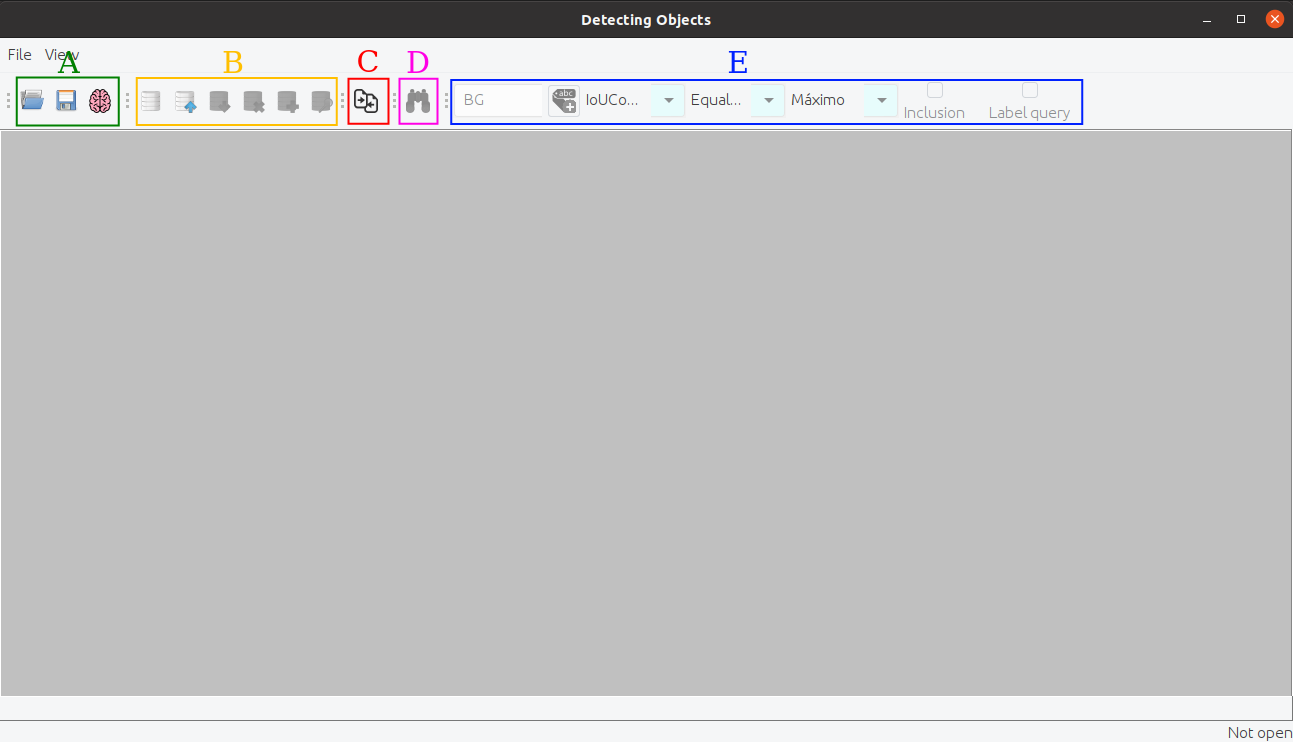
\includegraphics[width=1.0\textwidth]{ventanaprincipal}
  \caption{Ventana principal del prototipo.}
  \label{fig:ventanaprincipal}
\end{figure}

\begin{figure}[htpb]
  \centering
  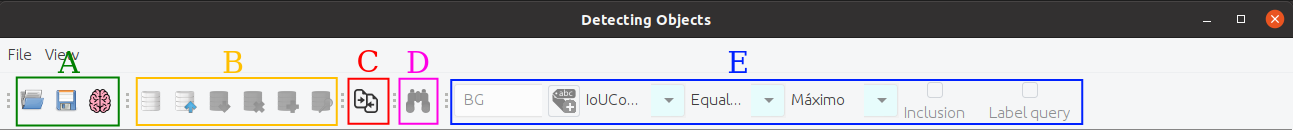
\includegraphics[width=1.0\textwidth]{barraherramientas}
  \caption{Barra de herramientas del prototipo.}
  \label{fig:barraherramientas}
\end{figure}

Para simplificar la explicación, se agruparán los botones de acuerdo a funcionalidades.\\

\newpage

En la primera zona, marcada en verde y bajo la etiqueta A, se encuentran los botones relacionados con la entrada y salida de imágenes así como la funcionalidad de abrir el fichero de pesos de la red neuronal que queramos cargar.

\begin{enumerate}
\item El primer botón sirve para abrir imágenes, permitiendo la selección múltiple.
\item El segundo botón permite guardar la imagen seleccionada en el escritorio, siendo que si esta es la generada con la salida de la red neuronal también se almacenarán los puntos como si fueran parte de la propia imagen.
\item El tercer botón sirve para para abrir el fichero de pesos, con la extensión \emph{h5}, de la red neuronal que deseemos utilizar para generar las predicciones. Al cargar correctamente un fichero, habilitarán los botones de la zona D y E. Si realizamos click derecho, aparecerá las opciones de descriptores posibles a utilizar para la utilidad de la zona D, permitiendo la opción múltiple entre descriptores de color o la opción singular del descriptor por etiqueta. \autoref{fig:descriptorred}
\end{enumerate}

\begin{figure}[h]
  \centering
  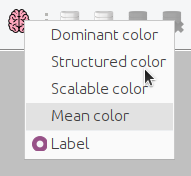
\includegraphics[width=0.4\textwidth]{descriptorred}
  \caption{Cargar pesos. Descriptores disponibles para la consulta de imágenes en el escritorio.}
  \label{fig:descriptorred}
\end{figure}

En la segunda zona, marcada en naranja y bajo la etiqueta B, se encuentran las opciones relacionadas con el sistema de bases de datos de la aplicación.

\begin{enumerate}
\item El primer botón corresponde a la opción de creación de una nueva base de datos, habilita el resto de botones relacionados con una base de datos. Al realizar click derecho, muestra las opciones de descriptores a utilizar con la nueva base de datos a crear o abrir, permitiendo la opción múltiple entre descriptores de color o la opción singular del descriptor por etiqueta.
\begin{figure}[h]
  \centering
  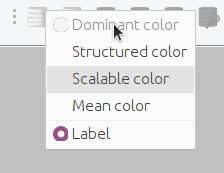
\includegraphics[width=0.4\textwidth]{descriptorbase}
  \caption{Abrir base de datos. Descriptores disponibles para la consulta de imágenes en la base de datos.}
  \label{fig:descriptorbase}
\end{figure}
\item El segundo botón sirve para abrir una de las bases de datos guardadas con anterioridad en el sistema, habilita el resto de botones relacionados con una base de datos.
\item El tercer botón corresponde a la opción de guardar la base de datos actual, permitiendo seleccionar el directorio de guardado y el nombre de la base de datos.
\item El cuarto botón sirve para cerrar sin guardar la base de datos actual.
\item El quinto botón sirve para añadir, bajo los descriptores seleccionados en la opción secundaria del primer botón, todas las imágenes del escritorio abiertas actualmente en la base de datos abierta.
\item El sexto botón sirve para comparar la imagen seleccionada con todas las imágenes almacenadas en la base de datos, bajo los descriptores seleccionados en las opciones disponibles en la opción secundaria del primer botón.
\end{enumerate}

En la tercera zona, marcada en rojo y bajo la etiqueta C, corresponde al botón de consulta entre las imágenes abiertas en el escritorio. Realiza una comparación, utilizando los descriptores marcados en el tercer botón de la zona A, de la imagen seleccionada con el resto de imágenes disponibles en el escritorio.\\

La tercera zona, con el color rosa y con la etiqueta D, corresponde a la realización de una predicción de la imagen seleccionada bajo la red neuronal cargada. \\

La cuarta zona corresponde a los parámetros de comparación a utilizar para los descriptores de etiquetas.
\begin{itemize}
\item El primer listado permite la selección de una etiqueta para la búsqueda por etiquetas en el caso de que esta opción este seleccionada. \autoref{fig:categories}
\begin{figure}[H]
  \centering
  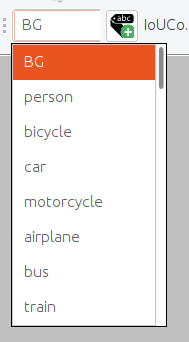
\includegraphics[width=0.2\textwidth]{categories}
  \caption{Lista de categorías disponibles.}
  \label{fig:categories}
\end{figure}
\item El segundo botón permite la selección múltiple de etiquetas para la búsqueda por etiquetas en caso de que está opción este seleccionada.
\item El tercer listado permite la selección del comparador a utilizar para la búsqueda por etiquetas con regiones, tanto para la consulta en base de datos como la consulta en escritorio. \autoref{fig:comparator}
\begin{figure}[H]
  \centering
  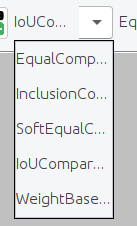
\includegraphics[width=0.2\textwidth]{comparator}
  \caption{Comparadores disponibles para la consulta por etiqueta.}
  \label{fig:comparator}
\end{figure}
\item El cuarto listado sirve para la seleccionar el comparador de etiquetas a utilizar con el \emph{IoUComparator}.\autoref{fig:equalcomparator}
\begin{figure}[H]
  \centering
  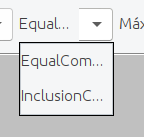
\includegraphics[width=0.2\textwidth]{equalcomparator}
  \caption{Comparación de etiquetas disponibles para el \emph{IoUComparator}.}
  \label{fig:equalcomparator}
\end{figure}
\item El quinto listado permite la selección de la operación de agregación a utilizar con el \emph{IoUComparator} y con \emph{WeightBasedComparator}. \autoref{fig:agregation}
\begin{figure}[H]
  \centering
  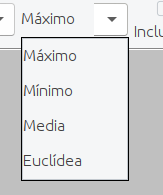
\includegraphics[width=0.2\textwidth]{agregation}
  \caption{Operaciones de agregación disponibles para el \emph{IouComparator} y el \emph{WeightBasedComparator}.}
  \label{fig:agregation}
\end{figure}
\item El sexto check permite distinguir si utilizamos un comparador de inclusión o uno de igualdad para el \emph{WeightBasedComparator}.
\item El séptimo, y último, check permite habilitar la búsqueda por etiquetas seleccionadas en el primer listado y en el segundo botón o deshabilitarla para realizar las consultas a través de la imagen seleccionada en el escritorio.
\end{itemize}

\chapter{Pruebas}
El objetivo principal de este capítulo es mostrar una serie de ejemplos de resultados del prototipo desarrollado, prestándole especial atención a los comparadores de \emph{RegionLabelDescriptor} al ser la principal característica del prototipo desarrollado.\\

\begin{figure}[htpb]
  \centering
  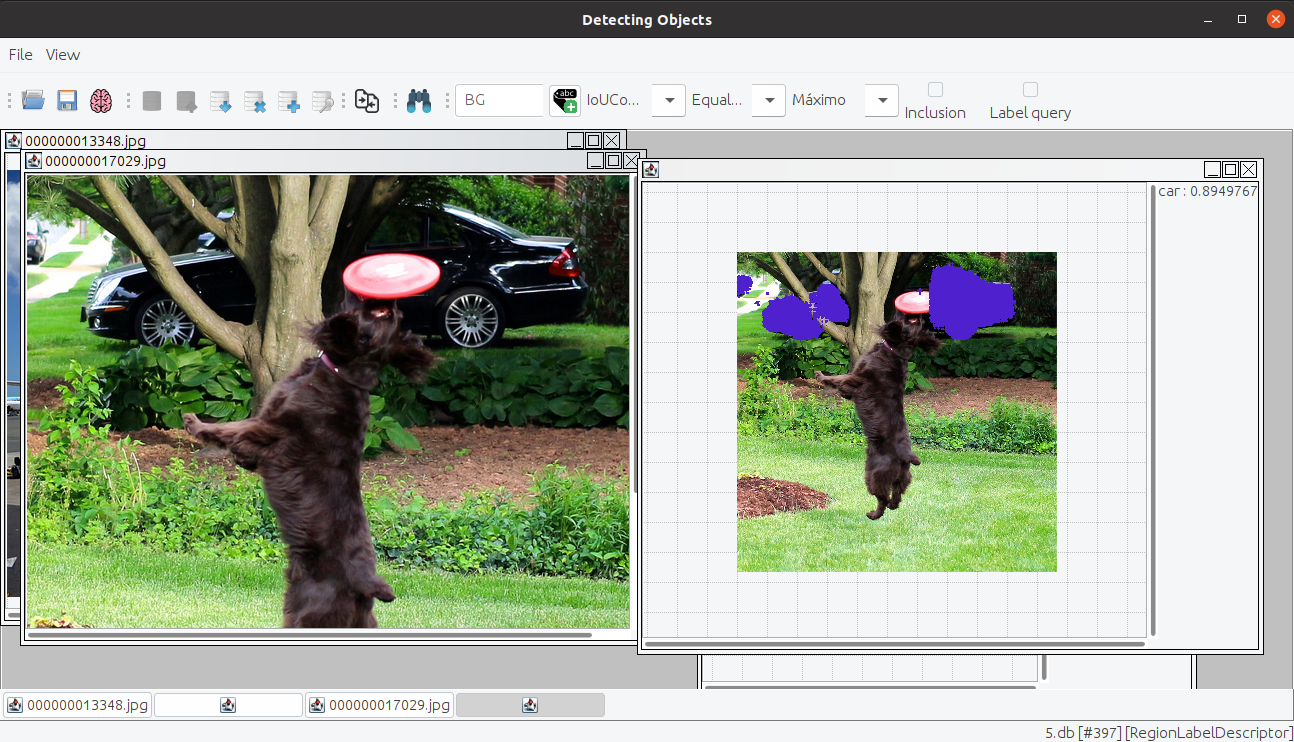
\includegraphics[width=0.9\textwidth]{DetectingObjects/pred1}
  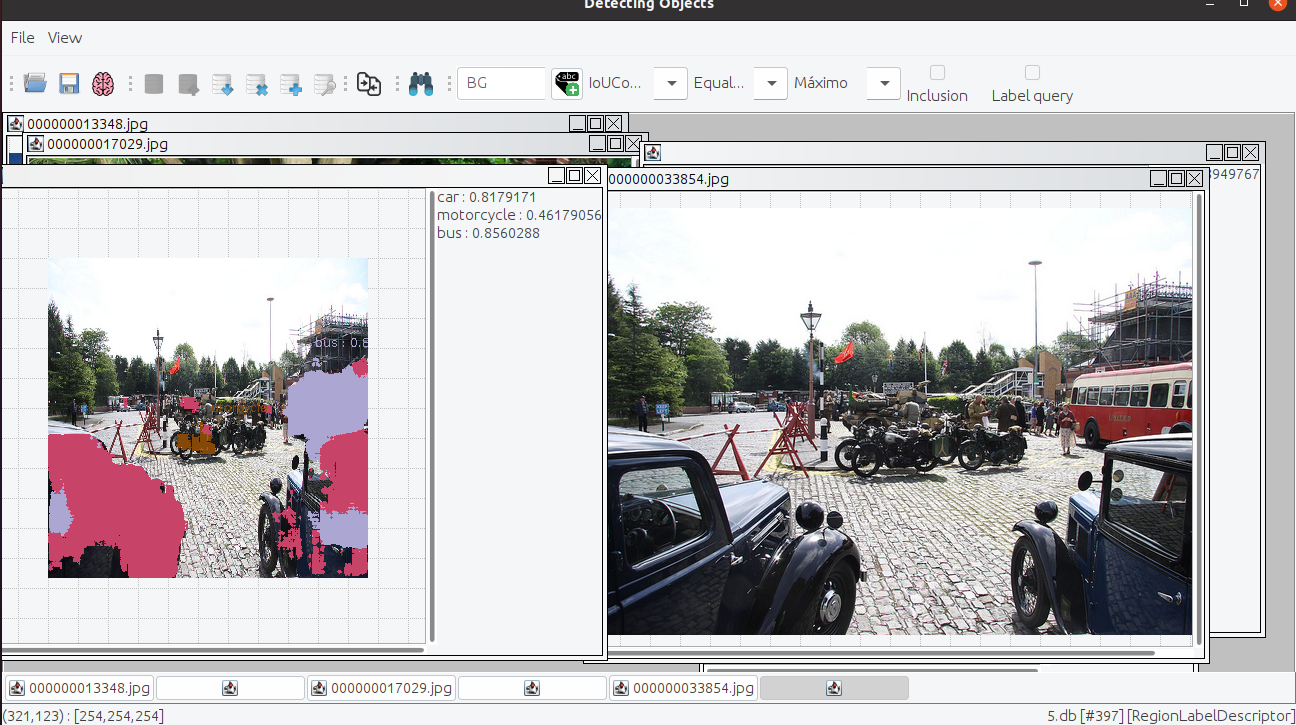
\includegraphics[width=0.9\textwidth]{DetectingObjects/pred2}
  \caption{Ejemplos de predicciones y el grado de confianza a partir de una función \emph{softmax} para el subconjunto de transportes.}
  \label{fig:pred}
\end{figure}

Para una de las bases de datos de tipo etiqueta, se han utilizado aquellas imágenes del conjunto de datos de validación de COCO \cite{COCO} que tienen etiquetas relacionadas con transportes y tienen un índice menor a 200162 puesto que se ha utilizado un fichero de pesos relacionado con \autoref{fig:ejec5}, en particular aquel punto donde se alcanza un menor valor de pérdida en el entrenamiento.\\

En particular, en \autoref{fig:pred} se pueden apreciar un par de ejemplos de predicciones de esta red neuronal, mostrándose con colores aleatorios las distintas categorías. La confianza en la predicción será el correspondiente resultado tras aplicar la función \emph{softmax} al valor medio entre los puntos marcados contabilizando todas las categorías para una determinada etiqueta.\\

Las otras bases de datos implementadas, utilizarán imágenes del conjunto de datos de validación de COCO \cite{COCO} y sin restricciones respecto a las categorías a las que tienen que pertenecer las imágenes. Estas bases de datos será las que tendrán descriptores relacionados con colores \autoref{fig:REC} y bases de datos de etiquetas que contemplen todas las categorías. En concreto se tendrá una base de datos que represente el entrenamiento \autoref{fig:ejec10}, en los cuáles algunos ejemplos de predicciones pueden ser vistos en \autoref{resultados}.\\

\begin{figure}[htpb]
  \centering
  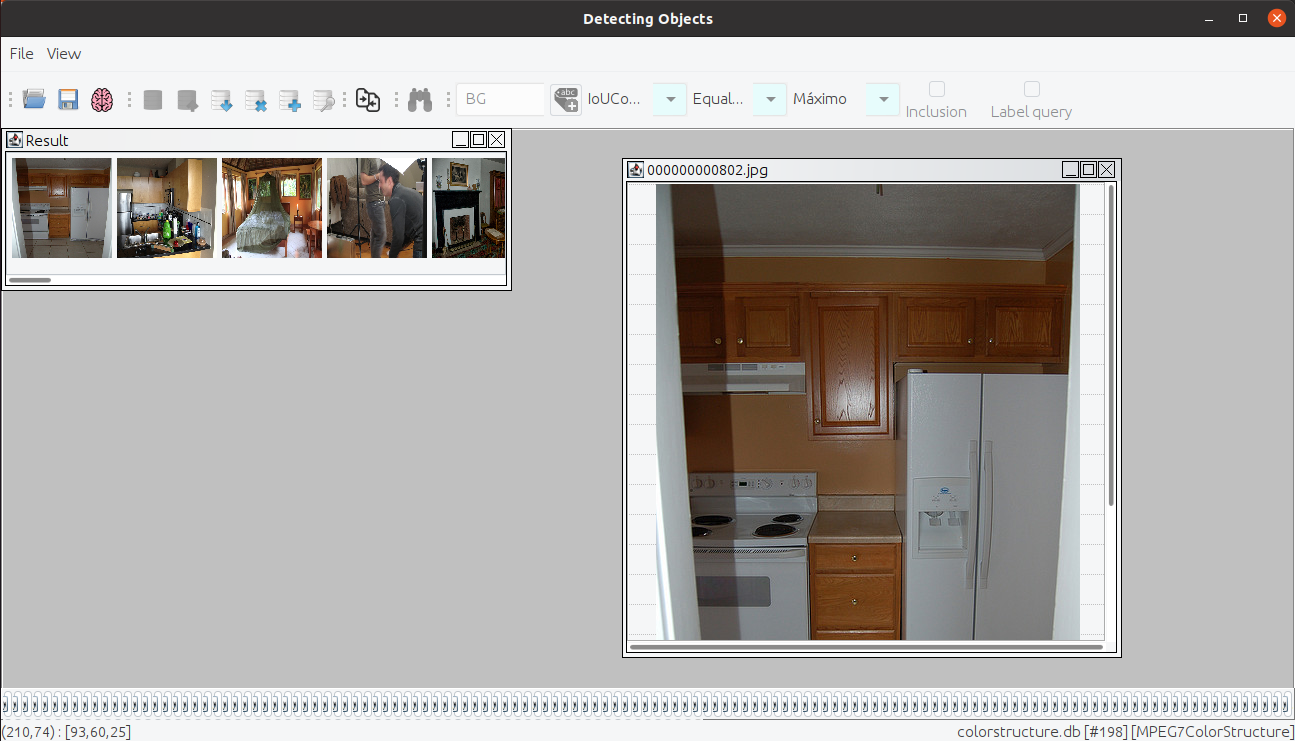
\includegraphics[width=0.9\textwidth]{DetectingObjects/REC}
  \caption{Ejemplo recuperación de imágenes basada en su color estructurado.}
  \label{fig:REC}
\end{figure}

Antes de mostrar de las distintas posibilidades de comparación existentes mediante la comparación de una imagen concreta, mostraremos los diferentes resultados obtenidos según la imagen que utilicemos para la búsqueda, manteniendo fijo el comparador. \autoref{fig:rec}\\

\begin{figure}[htpb]
  \centering
  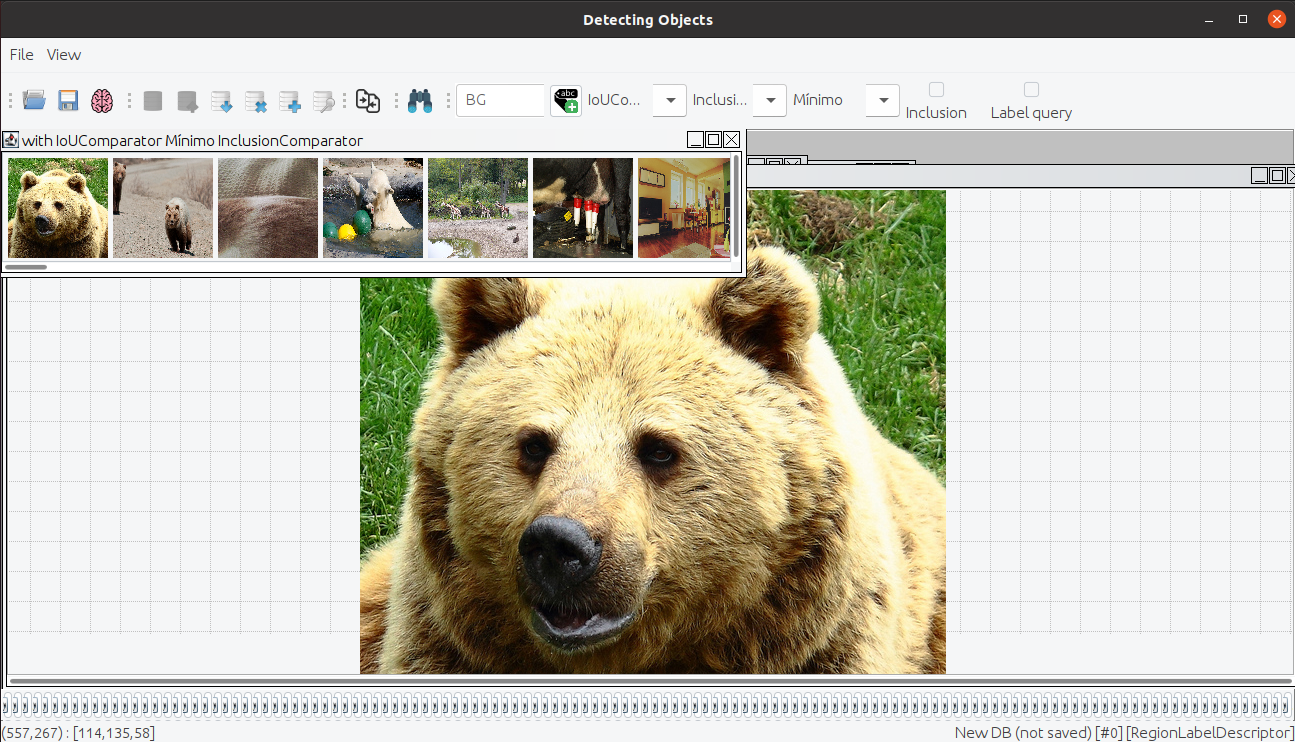
\includegraphics[width=0.9\textwidth]{DetectingObjects/rec}
  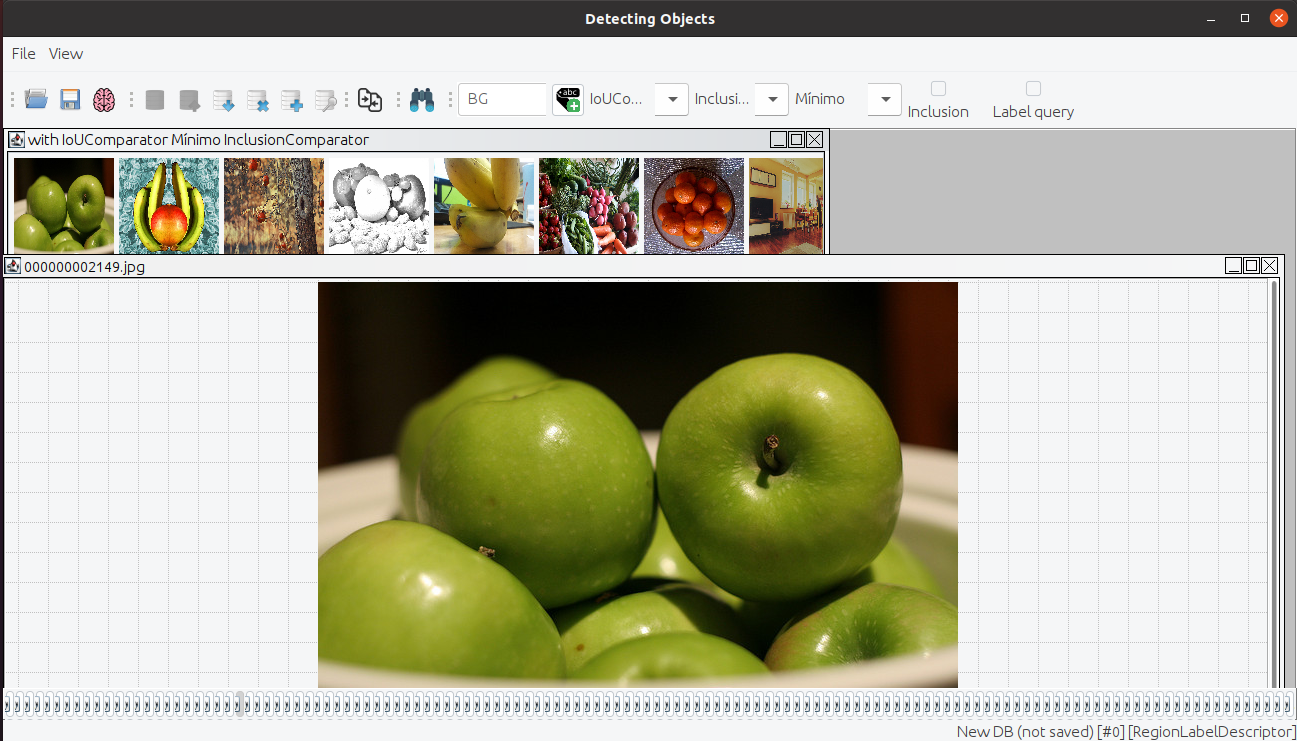
\includegraphics[width=0.9\textwidth]{DetectingObjects/rec1}
  \caption{Ejemplos recuperación de imágenes considerando todas las categorías.}
  \label{fig:rec}
\end{figure}

\newpage

A continuación, se fijará una imagen y se verá cómo varía el resultado dependiendo de qué comparador, y con qué parámetros, estemos utilizando. La idea es mostrar la recuperación de imágenes utilizando comparadores que únicamente miren la igualdad, inclusión o igualdad suave entre etiquetas o que tengan en cuenta también otros criterios como puede ser los pesos obtenidos a la hora de etiquetas las imágenes o la cantidad de píxeles coincidentes entre cada una de las etiquetas.\\

Primeramente, las imágenes resultado aparecerán ordenadas de menor a mayor resultado en la comparación, puesto que a mayor resultado más diferentes serán las imágenes de acuerdo al criterio de comparación seleccionado. En caso de compartir resultado, las imágenes aparecerán de acuerdo al orden en el que estén guardadas dentro de la propia base de datos.\\

Además, cabe destacar que se mostrarán todas y cada una de las imágenes almacenadas en la base de datos. Pudiéndose llegar a un punto en el que también aparezcan imágenes con distancia infinita, es decir, imágenes tan diferentes que no son comparables con el criterio utilizado.\\

En \autoref{fig:igualdad} se puede comprobar el resultado utilizando únicamente el comparador de igualdad \autoref{def:EqualComparator} entre categorías. En este caso el resultado esperado será tener una distancia con valor $0$ si la imagen comparada tiene únicamente las etiquetas ``coche'' y ``camión'', obteniendo $+\infty$ en caso de faltar alguna etiqueta o tener otra extra.\\
\begin{figure}[htpb]
  \centering
  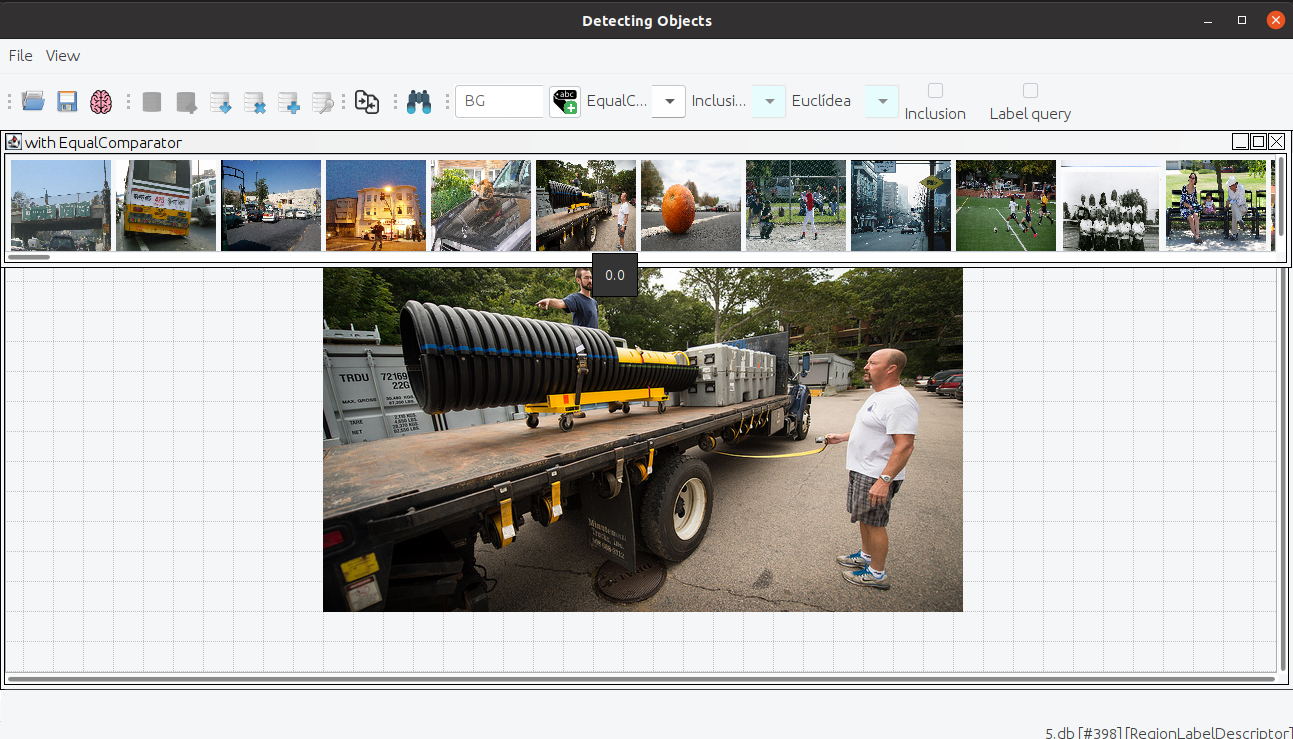
\includegraphics[width=0.9\textwidth]{DetectingObjects/IgualdadComparator}
  \caption{Comparador de igualdad entre etiquetas únicamente.}
  \label{fig:igualdad}
\end{figure}

En concreto, en esta relación se obtiene que desde la primera a la sexta imagen resultado tendremos imágenes que poseen únicamente las etiquetas ``coche'' y ``camión'' y por ello obtienen una distancia de $0.0$ con la imagen consultada. Estas imágenes ``iguales'', al no poder ordenarse por el valor de la predicción por compartir el mismo, serán ordenadas de acuerdo al orden en el que hayan sido almacenadas en la base de datos.\\

A partir de la séptima imagen, aquella que posee una ``naranja'', se tendrá distancia infinita con la imagen consultada. Es decir, de acuerdo al criterio de comparación seleccionado, son tan distintas de la imagen consultada que no pueden ser comparables.\\

Seguidamente, en \autoref{fig:inclusion} obtenemos el resultado tras el uso único del comparador de inclusión \autoref{def:InclusionComparator} entre etiquetas. Como se esperaba, se obtiene el valor $0$ si las categorías ``coche'' y ``camión'' están presentes en la imagen comparada de la base de datos y $+\infty$ si existe una carencia de alguna de ellas.\\

\begin{figure}[htpb]
  \centering
  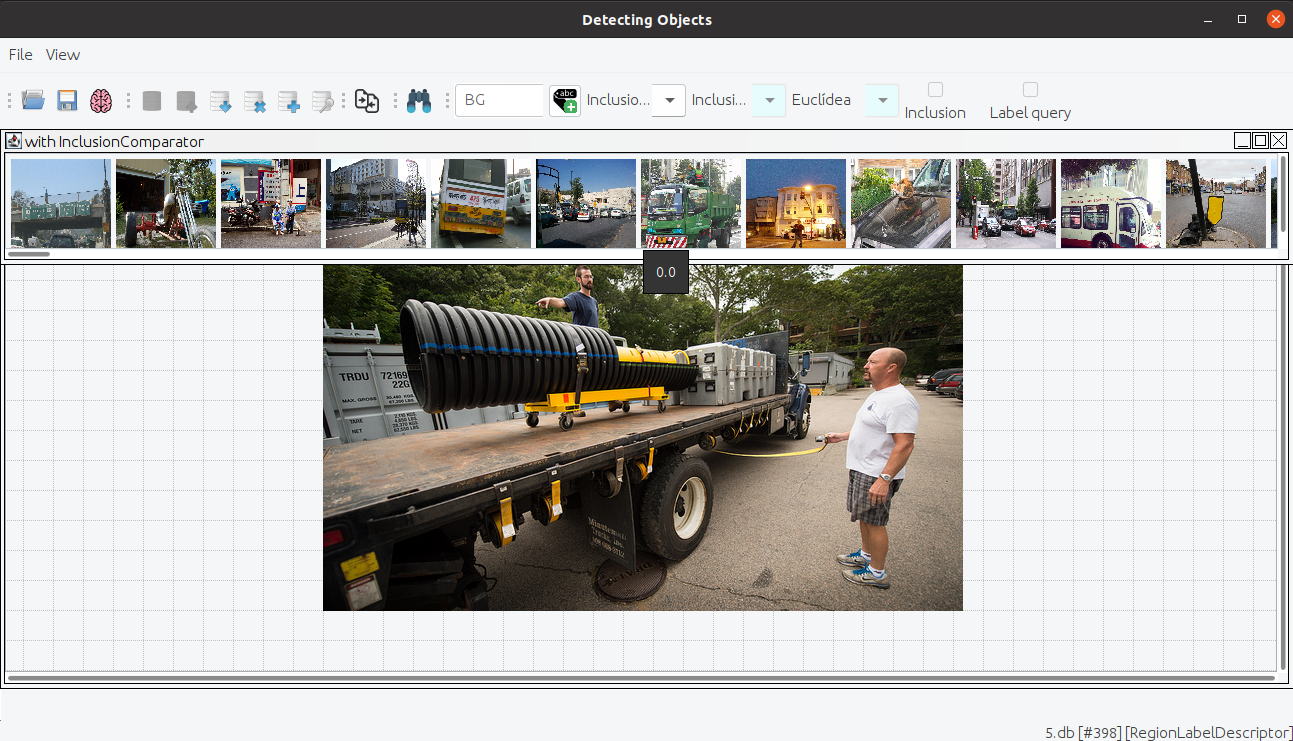
\includegraphics[width=0.9\textwidth]{DetectingObjects/InclusionComparator}
  \caption{Comparador de inclusión entre etiquetas únicamente.}
  \label{fig:inclusion}
\end{figure}

Finalizaremos los comparadores que comprueban exclusivamente las etiquetas con el comparador de ``igualdad suave'' \autoref{def:SoftEqualComparator}. La distancia será $0$ si sucede lo mismo que sucedía con el comparador de inclusión, añadiendo el hecho de que será también $0$ si la imagen a comparar posee únicamente las etiquetas ``coche'' o ``camión''. En cualquier caso será $+\infty$. Esto se puede apreciar en \autoref{fig:SoftEqualComparator}.\\

\begin{figure}[htpb]
  \centering
  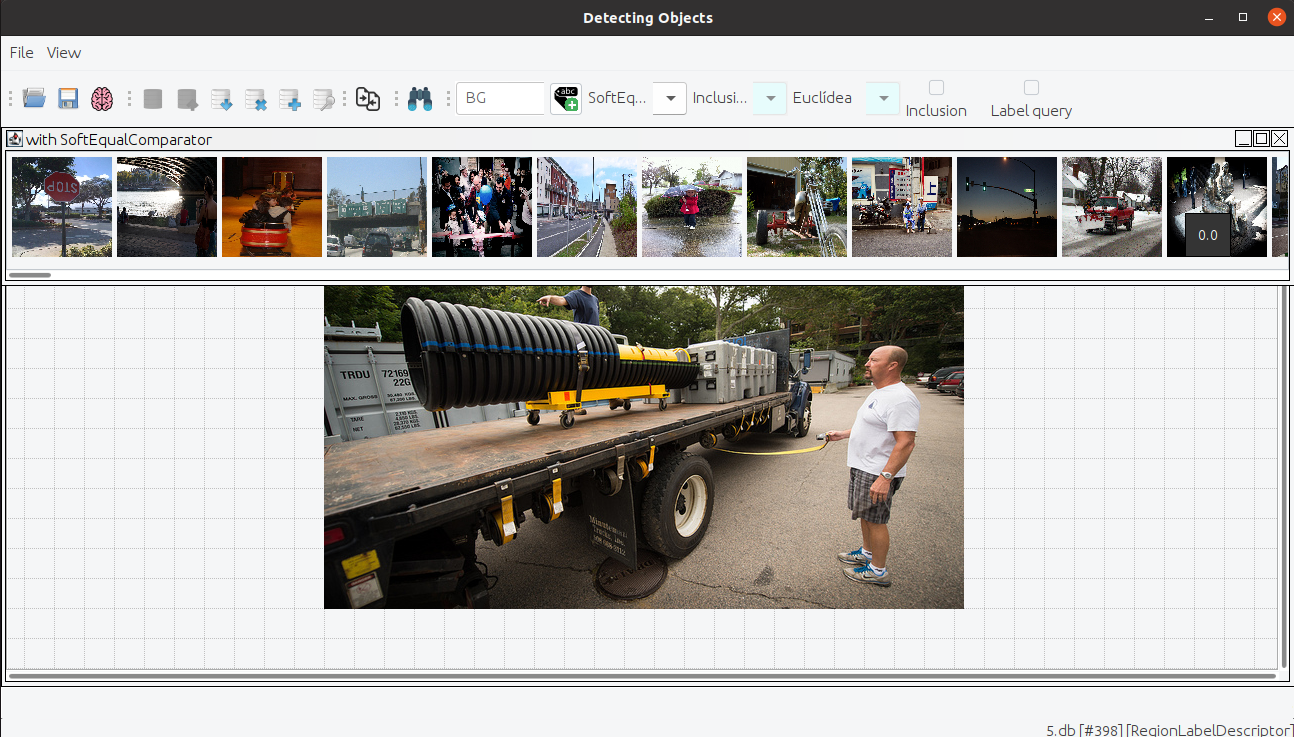
\includegraphics[width=0.9\textwidth]{DetectingObjects/SoftEqualComparator}
  \caption{Comparador de igualdad suave entre etiquetas únicamente.}
  \label{fig:SoftEqualComparator}
\end{figure}

\newpage
Continuaremos hablando del comparador basado en la intersección sobre la unión siendo el primer detalle fundamental que, dependiendo de si trabajamos con igualdad  o sólo inclusión, se devolverá la distancia infinita cuando la comparación por etiquetas inicial lo indique. Sin embargo, este no será el único caso en el que se devuelva dicha distancia infinita.\\

En particular, dadas una imagen seleccionada y una imagen a comparar, si existe una categoría en la imagen seleccionada tal que la intersección de todos los píxeles pertenecientes a estas categoría con los píxeles de la misma categoría de la imagen a comparar es vacía. Entonces, para esa categoría la distancia será infinita y, por tanto, por la propia definición de las funciones de agregación que mencionamos, las distancias totales bajo la operación de agregación del máximo, media aritmética o media geométrica devolverán $+\infty$.\\

Concretamente, si todas las intersecciones son nulas, la distancia bajo la operación del mínimo también será $+\infty$.\\

\begin{figure}[htpb]
  \centering
  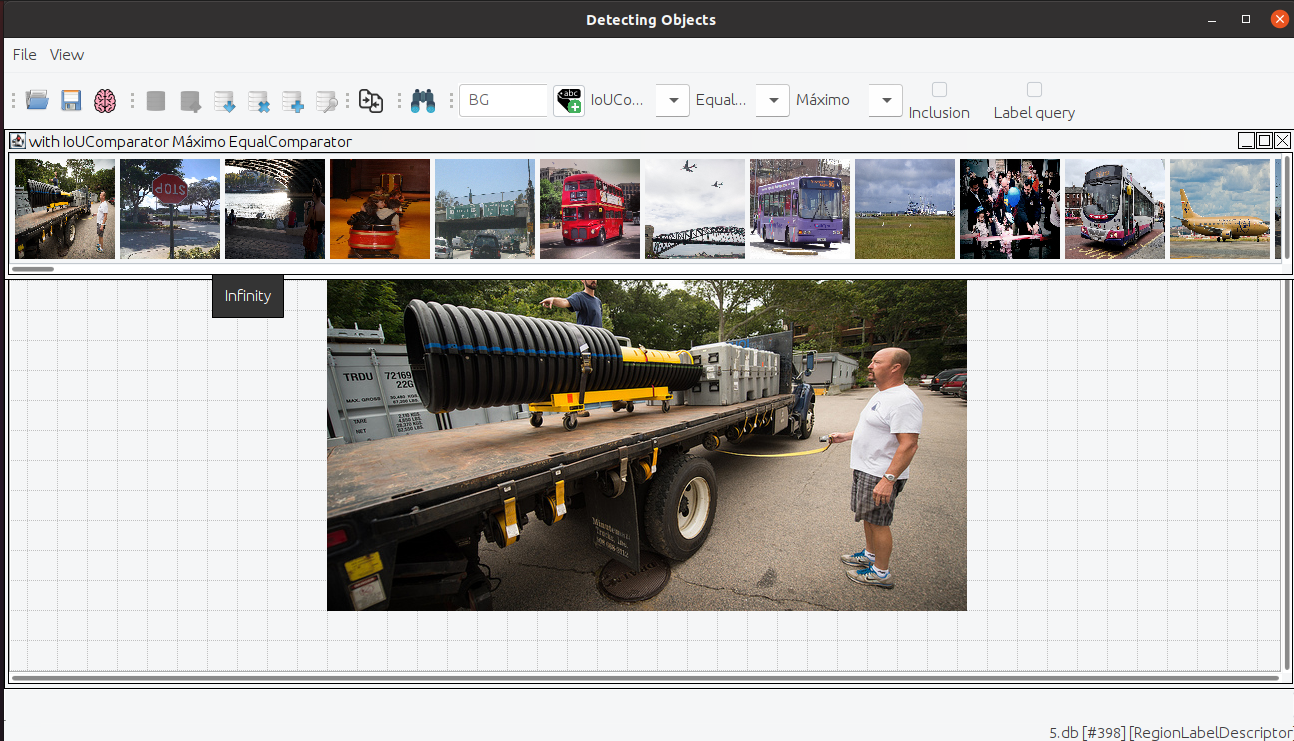
\includegraphics[width=1.0\textwidth]{DetectingObjects/IoUComparatorMaximoIgualdad}
  \caption{Comparador basado en IoU con igualdad entre etiquetas y operación del máximo como agregación entre etiquetas.}
  \label{fig:IoUComparatorMaximoIgualdad}
\end{figure}

\begin{figure}[htpb]
  \centering
  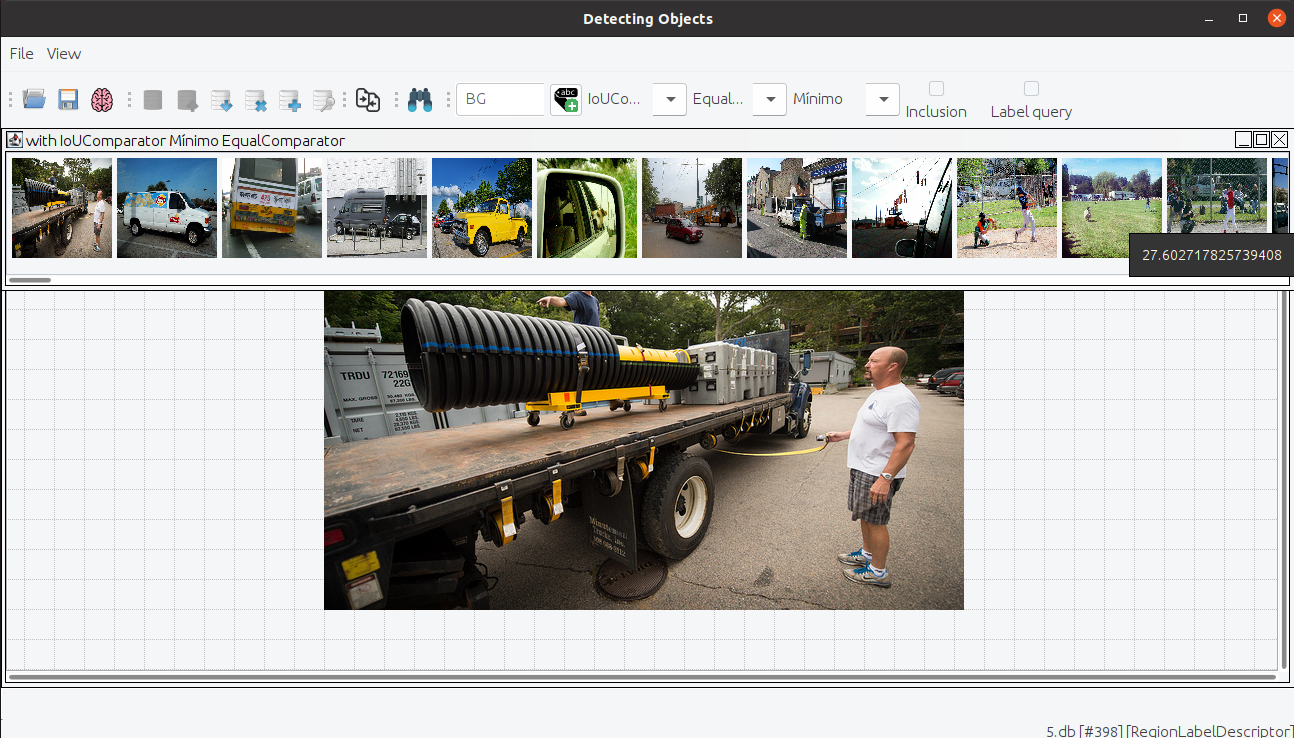
\includegraphics[width=1.0\textwidth]{DetectingObjects/IoUComparatorMinimoIgualdad}
  \caption{Comparador basado en IoU con igualdad entre etiquetas y operación del mínimo como agregación entre etiquetas.}
  \label{fig:IoUComparatorMinimoIgualdad}
\end{figure}

\begin{figure}[htpb]
  \centering
  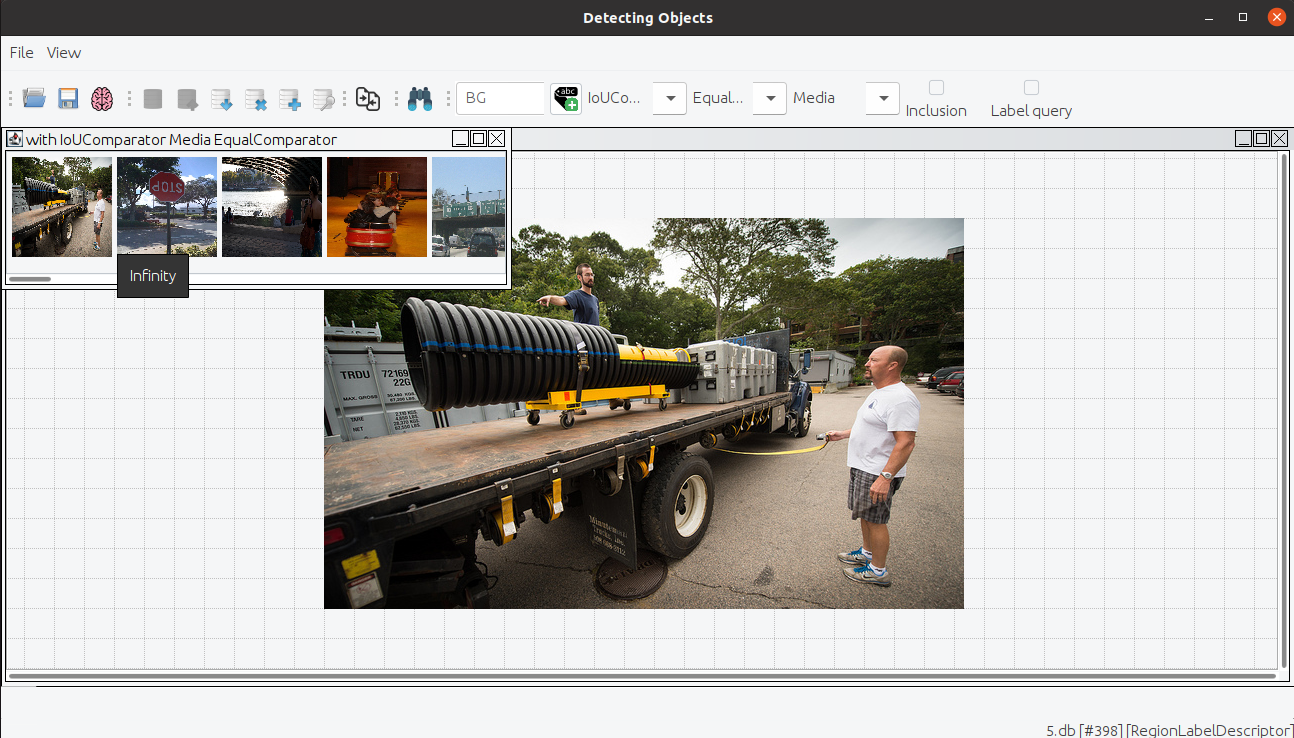
\includegraphics[width=1.0\textwidth]{DetectingObjects/IoUComparatorMediaIgualdad}
  \caption{Comparador basado en IoU con igualdad entre etiquetas y con la medía aritmética como agregación entre etiquetas.}
  \label{fig:IoUComparatorMediaIgualdad}
\end{figure}

\begin{figure}[htpb]
  \centering
  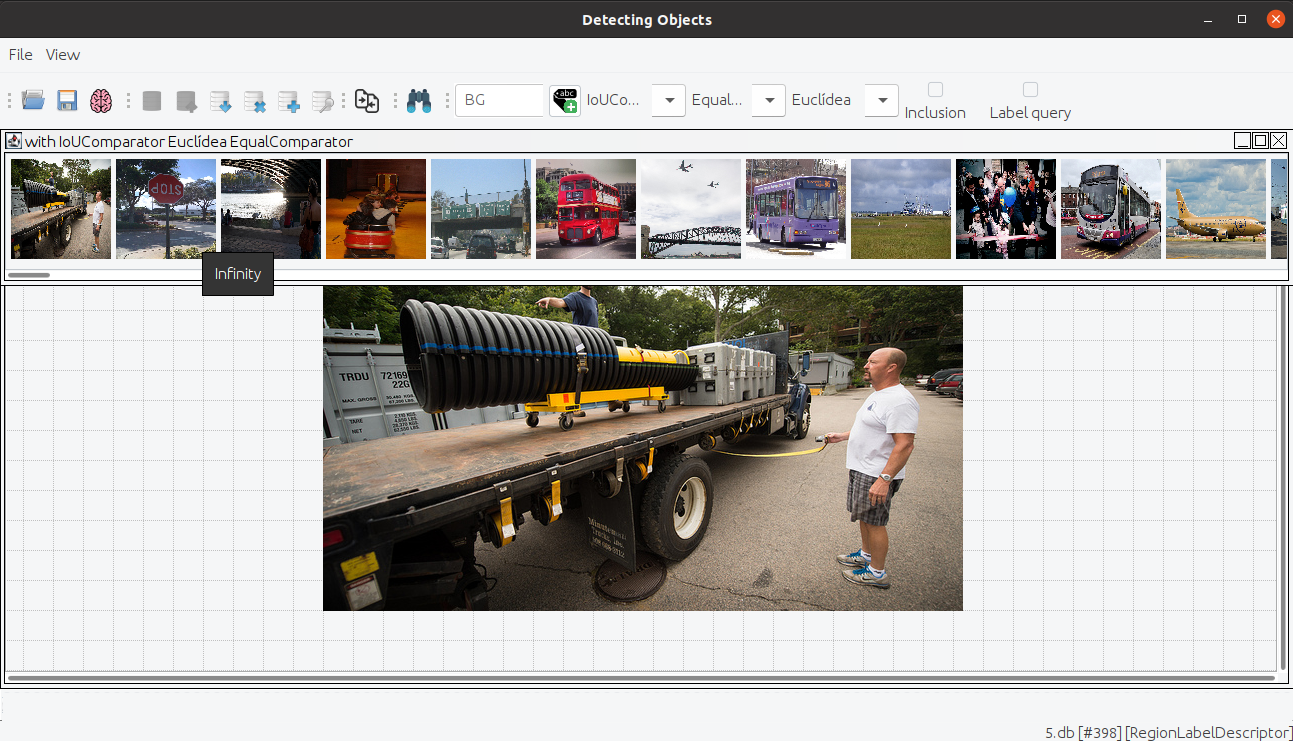
\includegraphics[width=1.0\textwidth]{DetectingObjects/IoUComparatorEuclideaIgualdad}
  \caption{Comparador basado en IoU con igualdad entre etiquetas y con la media euclídea como agregación entre etiquetas.}
  \label{fig:IoUComparatorEuclideaIgualdad}
\end{figure}

\begin{figure}[htpb]
  \centering
  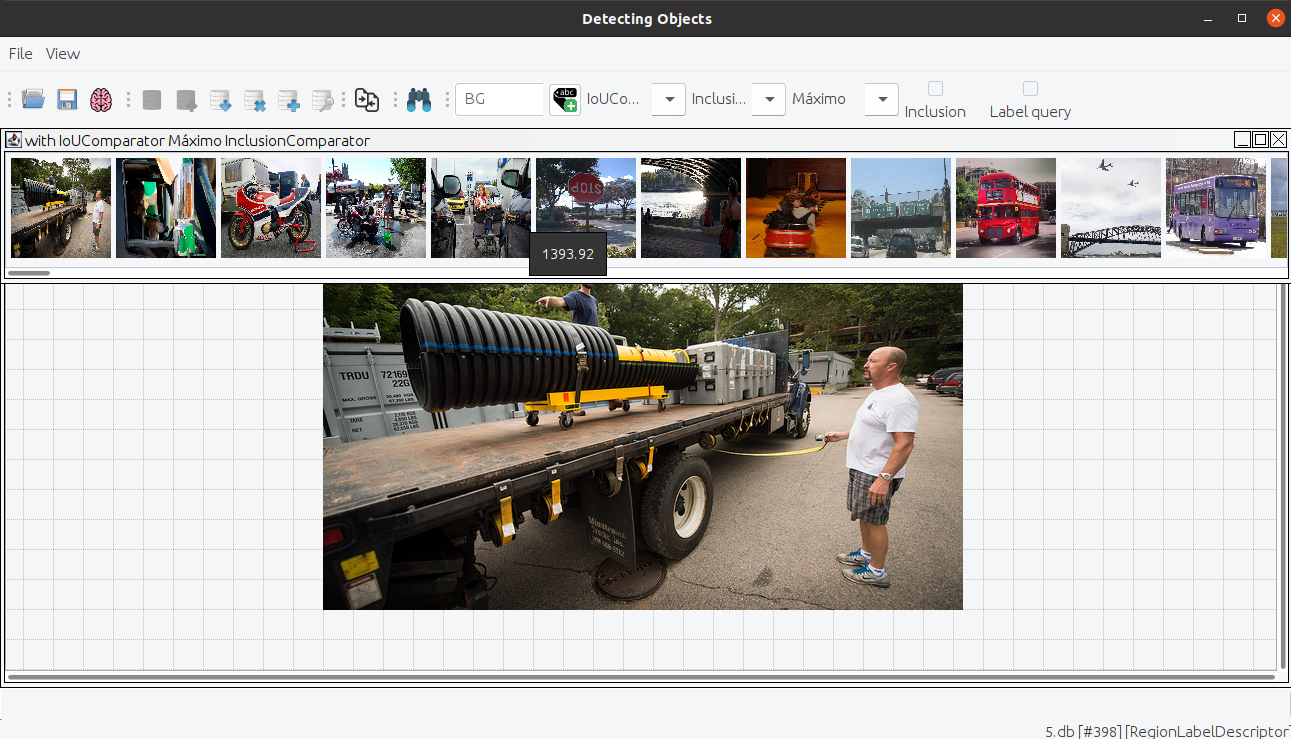
\includegraphics[width=1.0\textwidth]{DetectingObjects/IoUComparatorMaximoInclusion}
  \caption{Comparador basado en IoU con inclusión entre etiquetas y operación del máximo como agregación entre etiquetas.}
  \label{fig:IoUComparatorMaximoInclusion}
\end{figure}

\begin{figure}[htpb]
  \centering
  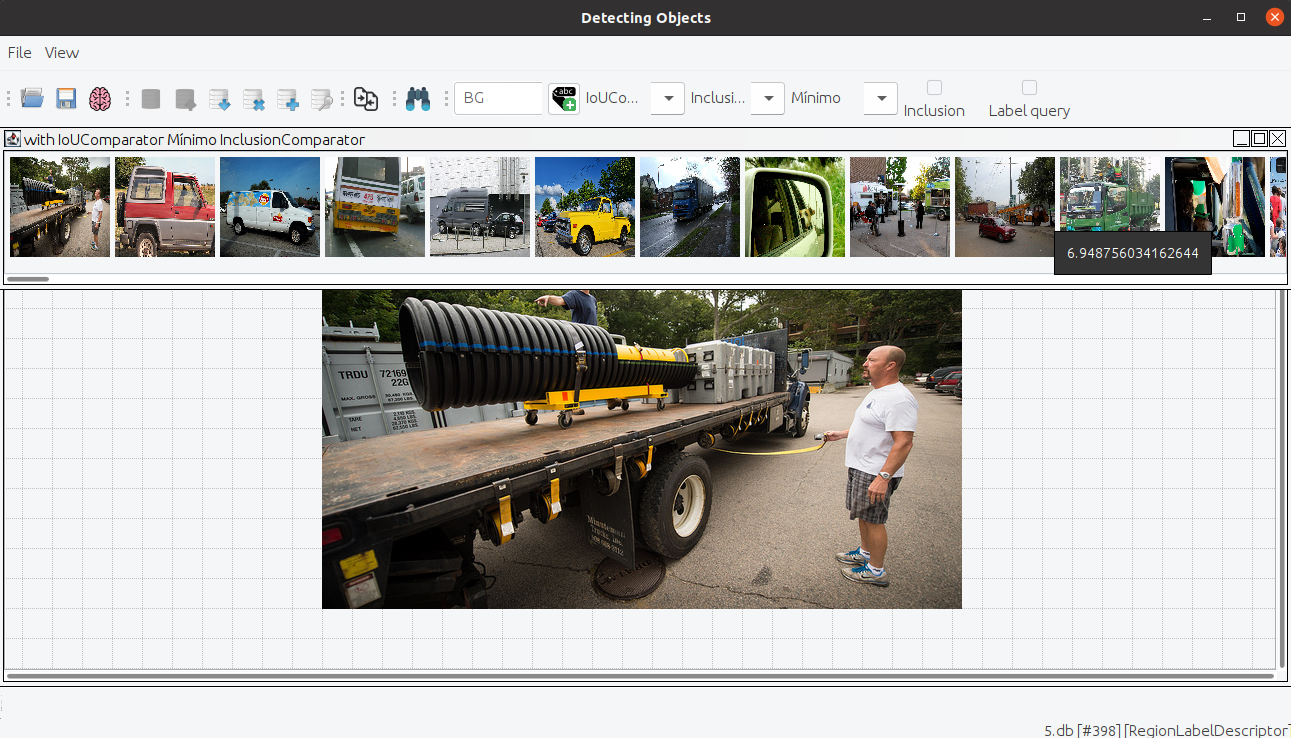
\includegraphics[width=1.0\textwidth]{DetectingObjects/IoUComparatorMinimoInclusion}
  \caption{Comparador basado en IoU con inclusión entre etiquetas y operación del mínimo como agregación entre etiquetas.}
  \label{fig:IoUComparatorMinimoInclusion}
\end{figure}

\begin{figure}[htpb]
  \centering
  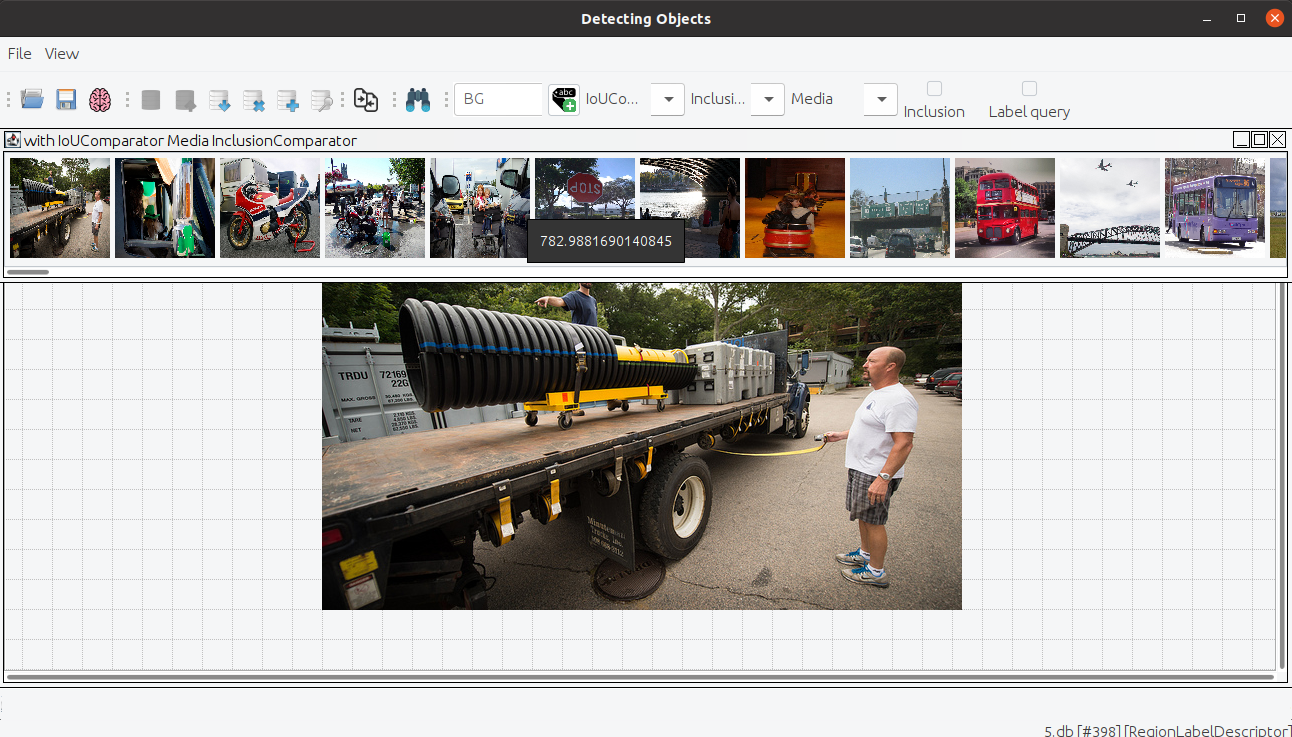
\includegraphics[width=1.0\textwidth]{DetectingObjects/IoUComparatorMediaInclusion}
  \caption{Comparador basado en IoU con inclusión entre etiquetas y con la medía aritmética como agregación entre etiquetas.}
  \label{fig:IoUComparatorMediaInclusion}
\end{figure}

\begin{figure}[htpb]
  \centering
  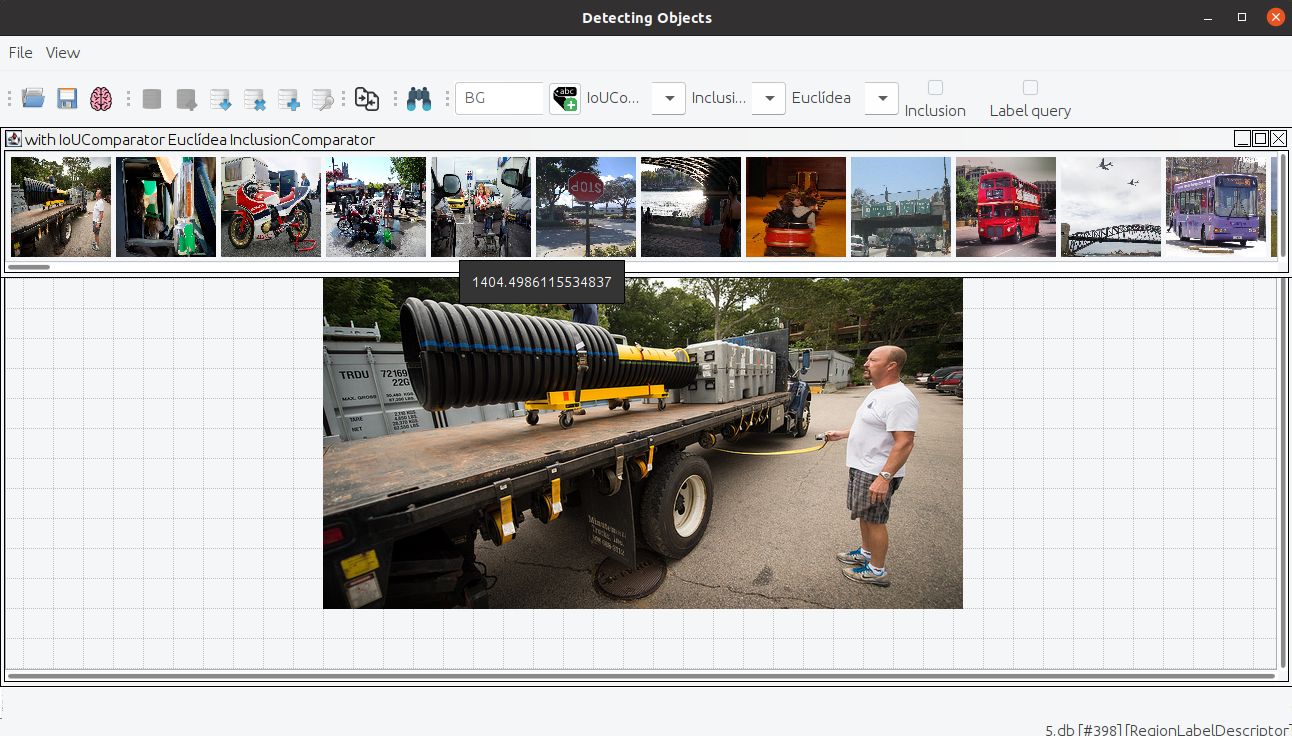
\includegraphics[width=1.0\textwidth]{DetectingObjects/IoUComparatorEuclideaInclusion}
  \caption{Comparador basado en IoU con inclusión entre etiquetas y con la media euclídea como agregación entre etiquetas.}
  \label{fig:IoUComparatorEuclideaInclusion}
\end{figure}

\newpage
Como último tipo de comparador con etiquetas, el comparador basado en pesos \autoref{def:WeightBasedComparator} tendrá el valor $+\infty$ únicamente cuando la comparación de igualdad(\autoref{fig:WeightBasedComparatorMaximoIgualdad}, \autoref{fig:WeightBasedComparatorMinimoIgualdad}, \autoref{fig:WeightBasedComparatorMediaIgualdad}, \autoref{fig:WeightBasedComparatorEuclideaIgualdad}) o inclusión(\autoref{fig:WeightBasedComparatorMaximoInclusion}, \autoref{fig:WeightBasedComparatorMinimoInclusion}, \autoref{fig:WeightBasedComparatorMediaInclusion}, \autoref{fig:WeightBasedComparatorEuclideaInclusion}) seleccionada marque este valor, mientras tanto retornará el valor marcado por la operación de agregación seleccionada.\\

\begin{figure}[htpb]
  \centering
  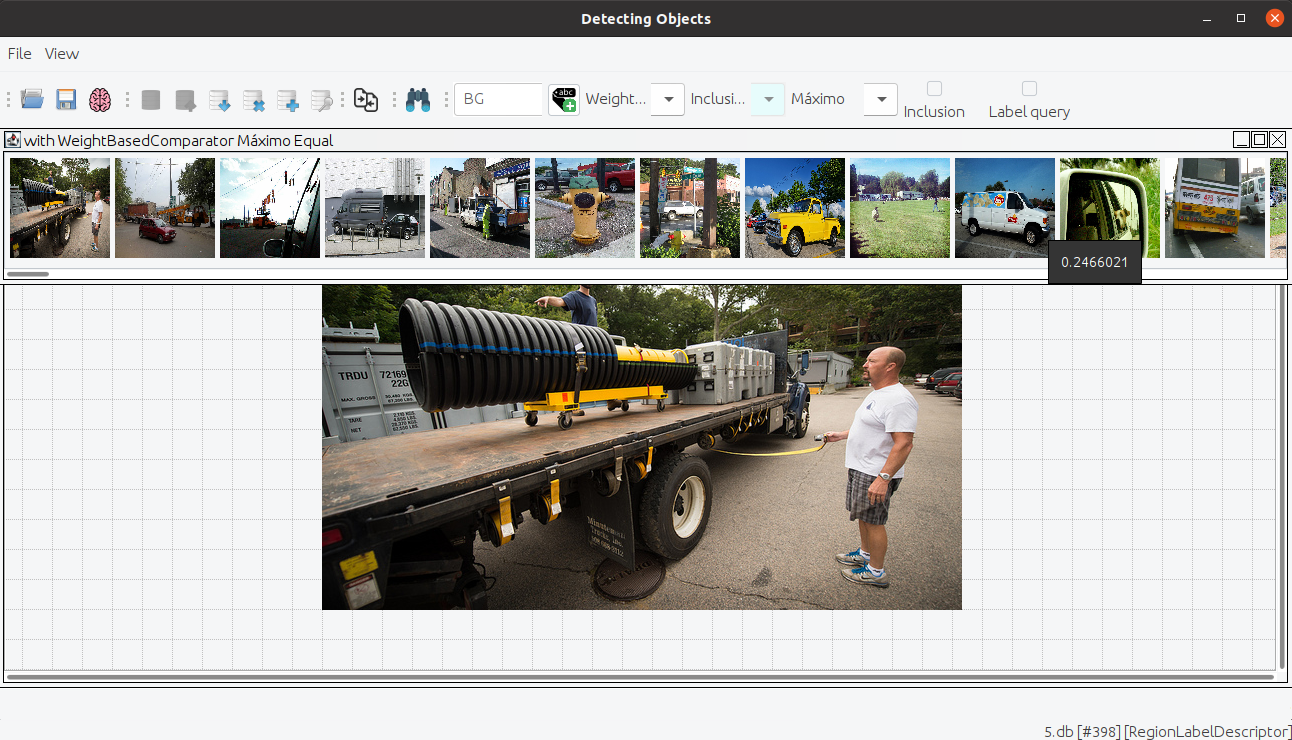
\includegraphics[width=1.0\textwidth]{DetectingObjects/WeightBasedComparatorMaximoIgualdad}
  \caption{Comparador basado en pesos con igualdad entre etiquetas y operación del máximo como agregación entre pesos.}
  \label{fig:WeightBasedComparatorMaximoIgualdad}
\end{figure}

\begin{figure}[htpb]
  \centering
  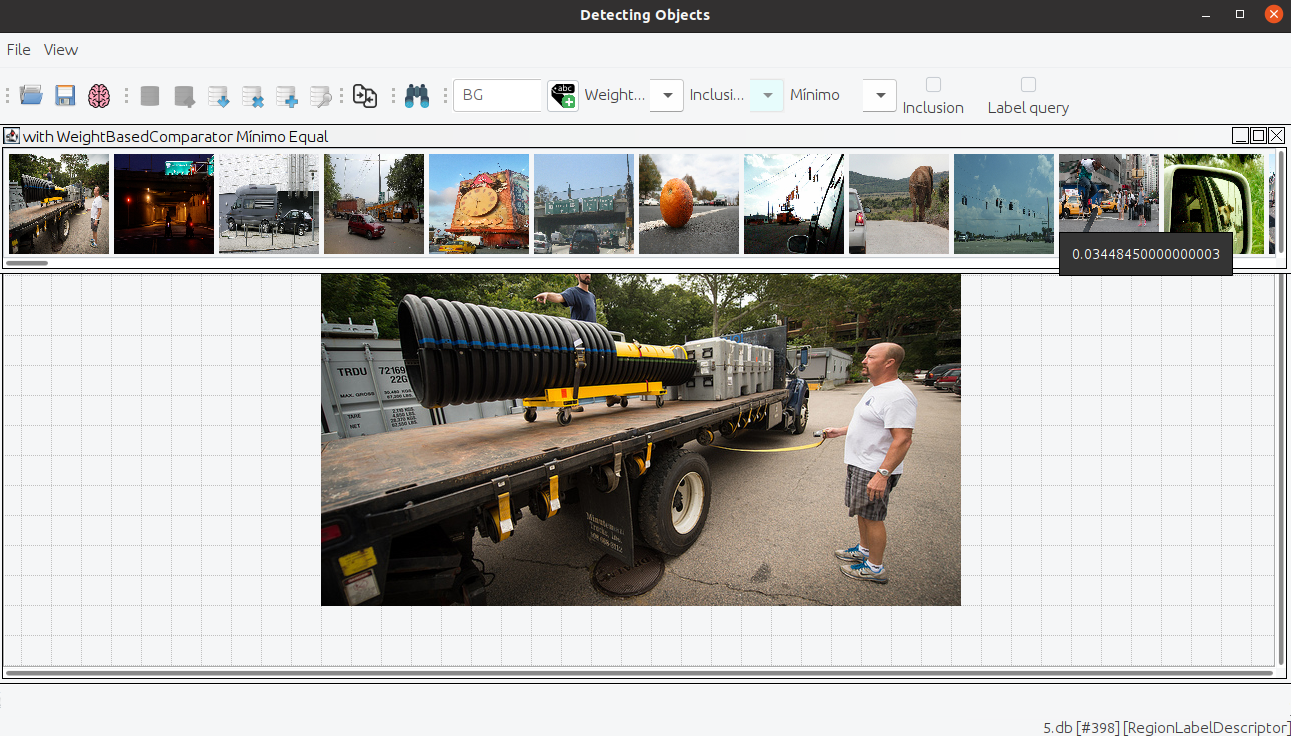
\includegraphics[width=1.0\textwidth]{DetectingObjects/WeightBasedComparatorMinimoIgualdad}
  \caption{Comparador basado en pesos con igualdad entre etiquetas y operación del mínimo como agregación entre pesos.}
  \label{fig:WeightBasedComparatorMinimoIgualdad}
\end{figure}

\begin{figure}[htpb]
  \centering
  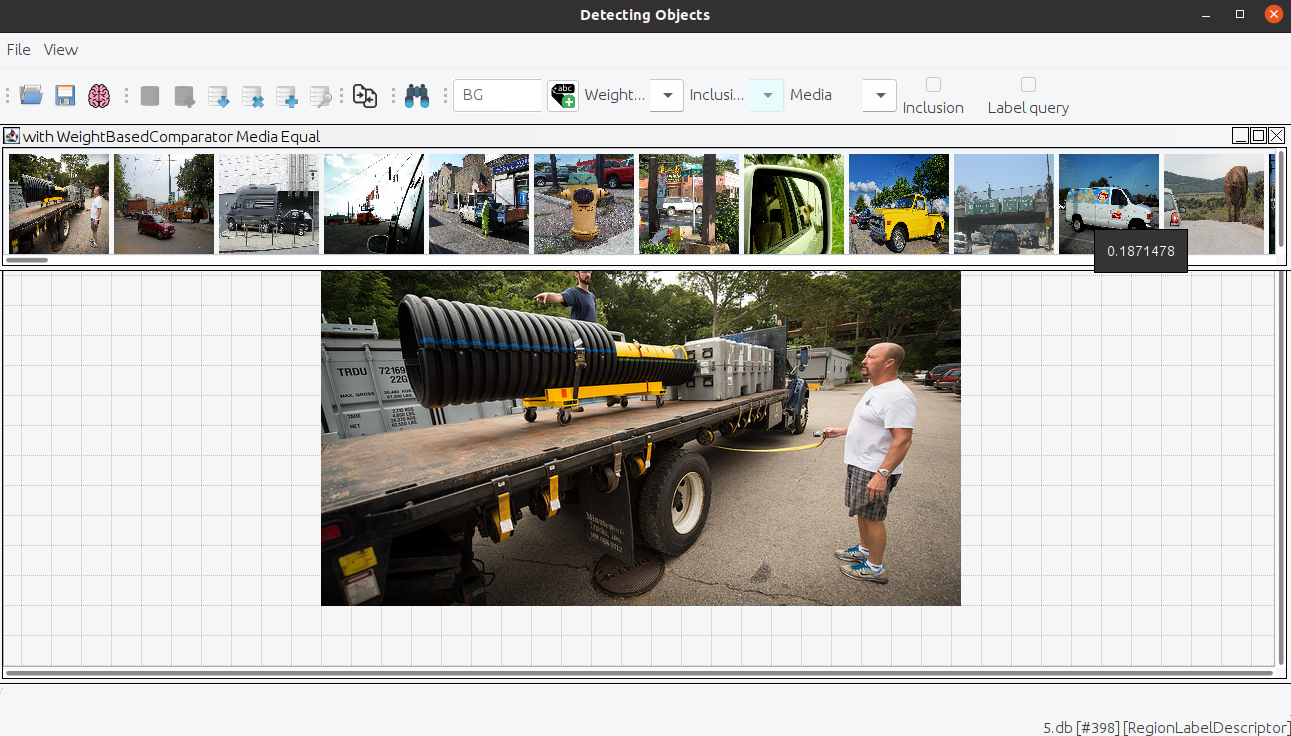
\includegraphics[width=1.0\textwidth]{DetectingObjects/WeightBasedComparatorMediaIgualdad}
  \caption{Comparador basado en pesos con igualdad entre etiquetas y con la medía aritmética como agregación entre pesos.}
  \label{fig:WeightBasedComparatorMediaIgualdad}
\end{figure}

\begin{figure}[htpb]
  \centering
  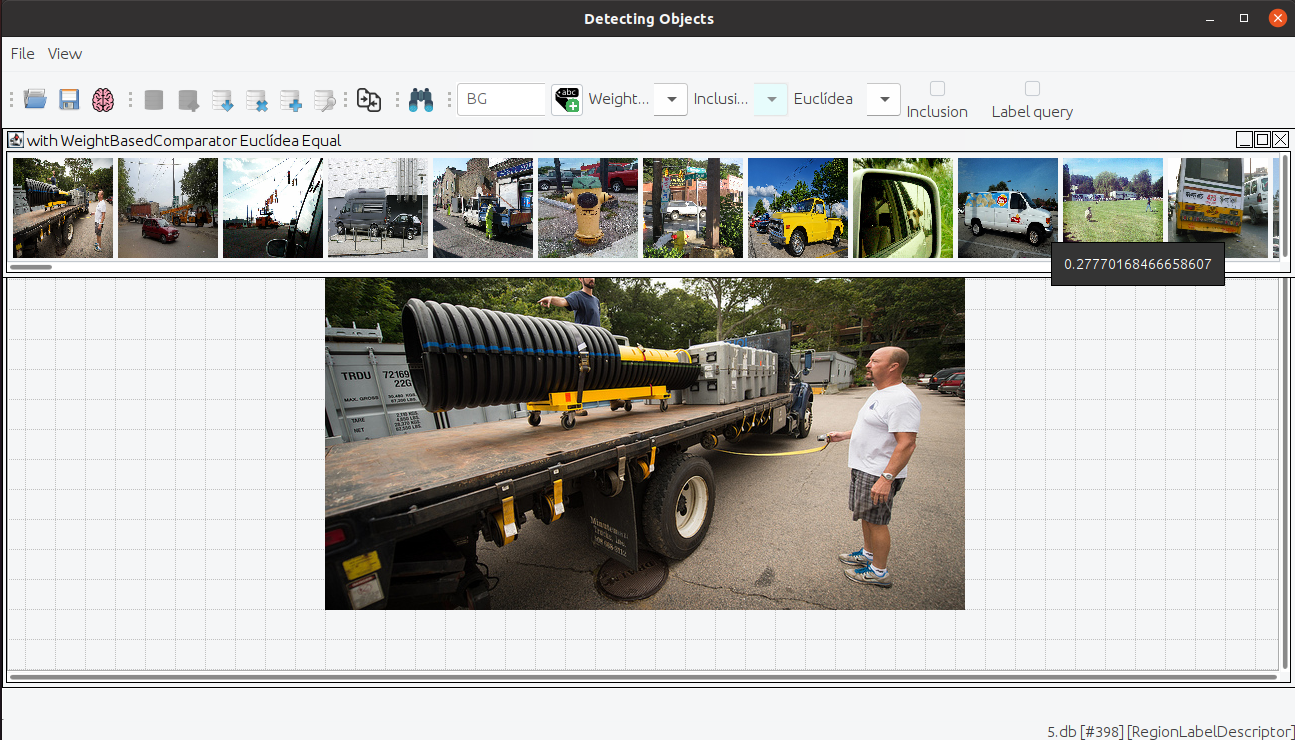
\includegraphics[width=1.0\textwidth]{DetectingObjects/WeightBasedComparatorEuclideaIgualdad}
  \caption{Comparador basado en pesos con igualdad entre etiquetas y con la media euclídea como agregación entre pesos.}
  \label{fig:WeightBasedComparatorEuclideaIgualdad}
\end{figure}

\begin{figure}[htpb]
  \centering
  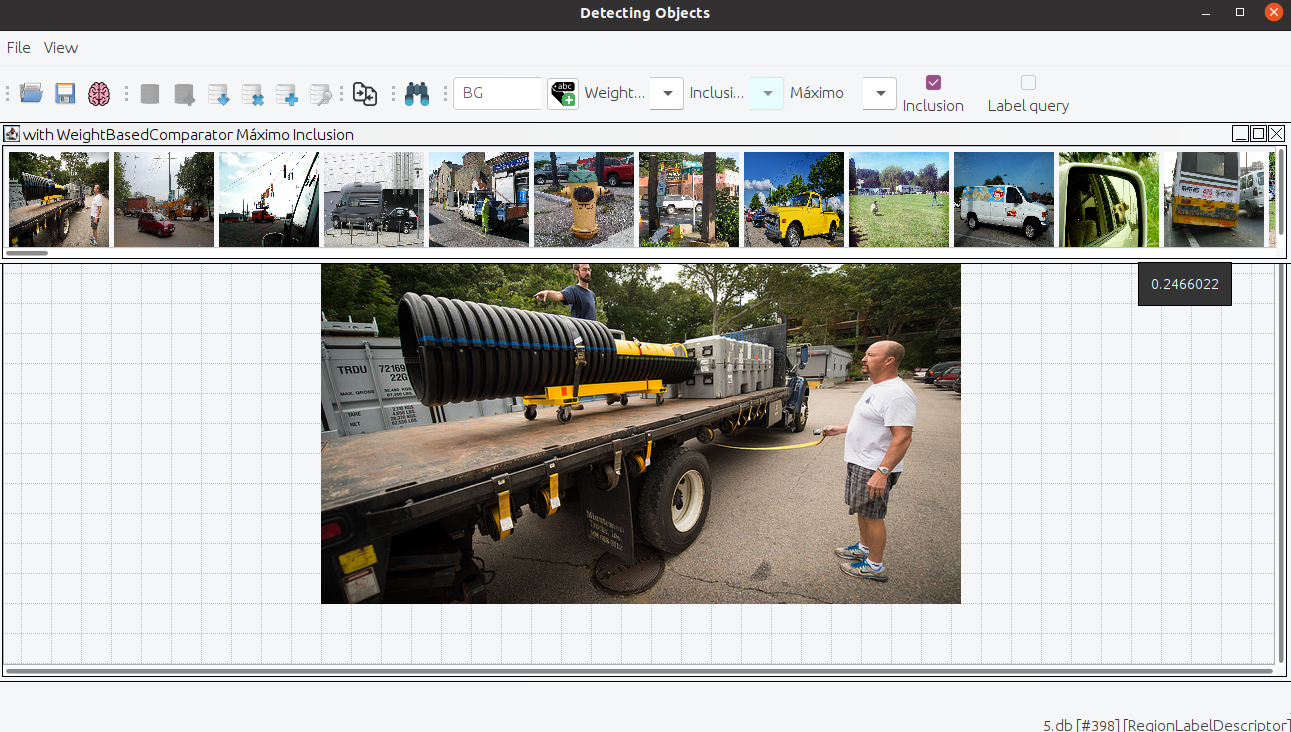
\includegraphics[width=1.0\textwidth]{DetectingObjects/WeightBasedComparatorMaximoInclusion}
  \caption{Comparador basado en pesos con inclusión entre etiquetas y operación del máximo como agregación entre pesos.}
  \label{fig:WeightBasedComparatorMaximoInclusion}
\end{figure}

\begin{figure}[htpb]
  \centering
  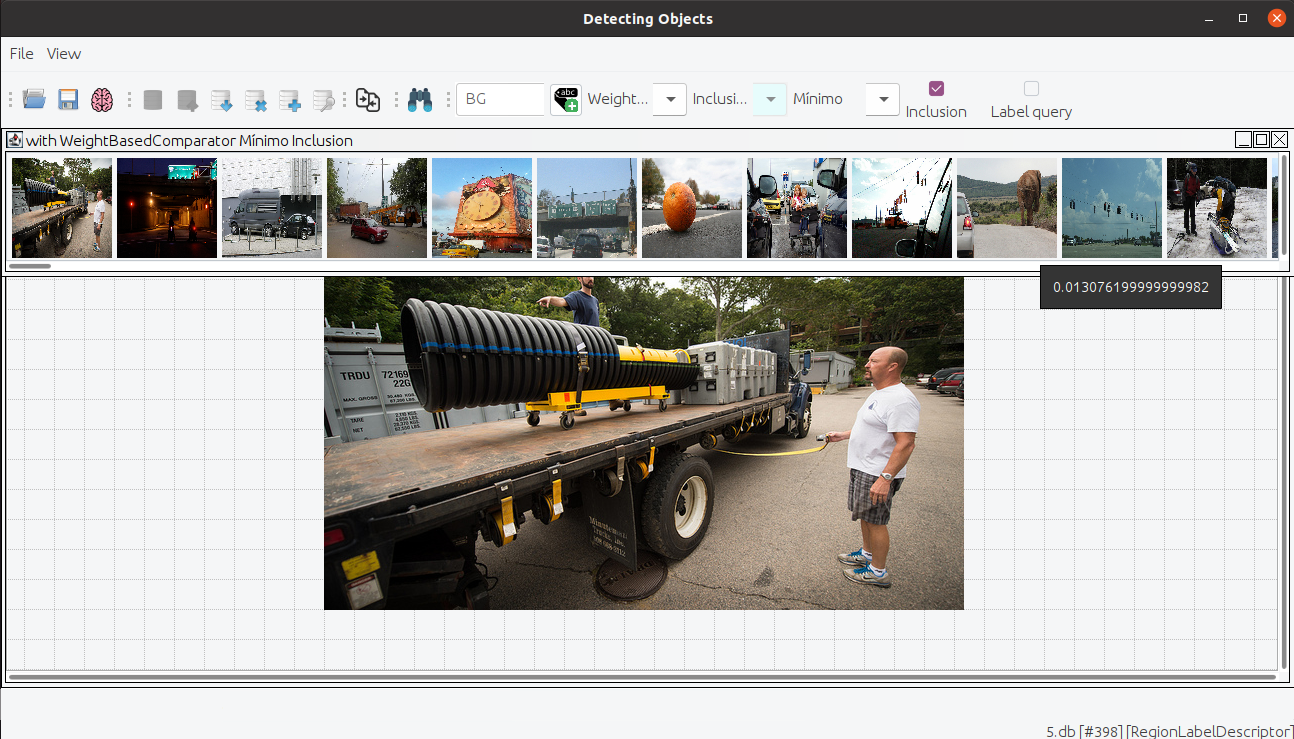
\includegraphics[width=1.0\textwidth]{DetectingObjects/WeightBasedComparatorMinimoInclusion}
  \caption{Comparador basado en pesos con inclusión entre etiquetas y operación del mínimo como agregación entre pesos.}
  \label{fig:WeightBasedComparatorMinimoInclusion}
\end{figure}

\begin{figure}[htpb]
  \centering
  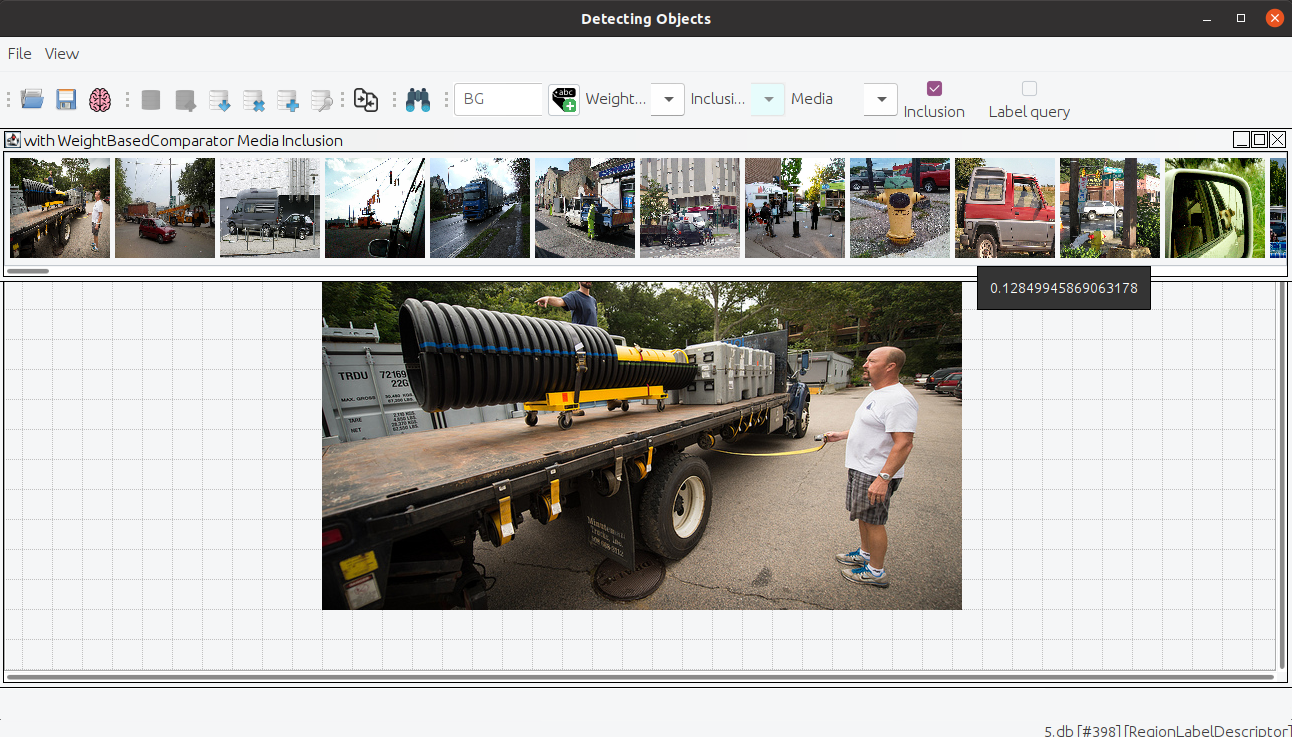
\includegraphics[width=1.0\textwidth]{DetectingObjects/WeightBasedComparatorMediaInclusion}
  \caption{Comparador basado en pesos con inclusión entre etiquetas y con la medía aritmética como agregación entre pesos.}
  \label{fig:WeightBasedComparatorMediaInclusion}
\end{figure}

\begin{figure}[htpb]
  \centering
  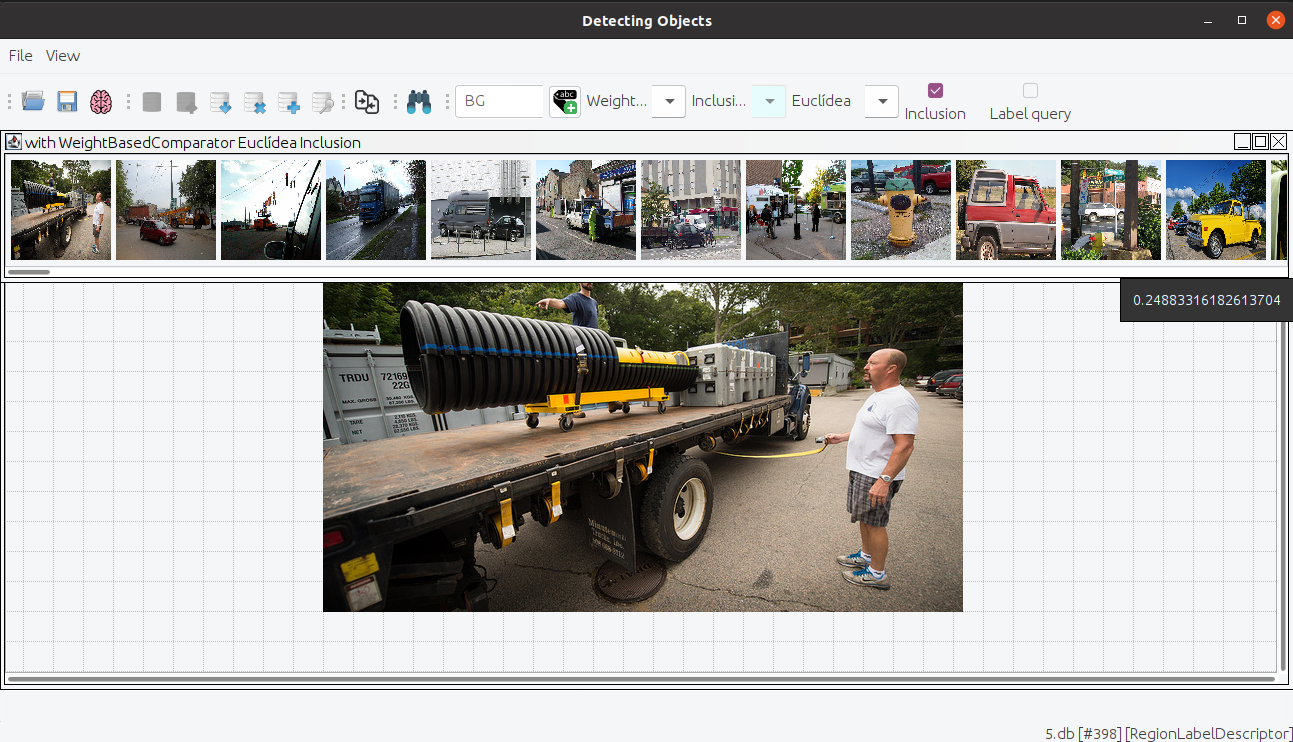
\includegraphics[width=1.0\textwidth]{DetectingObjects/WeightBasedComparatorEuclideaInclusion}
  \caption{Comparador basado en pesos con inclusión entre etiquetas y con la media euclídea como agregación entre pesos.}
  \label{fig:WeightBasedComparatorEuclideaInclusion}
\end{figure}

\part{Conclusiones del proyecto}
\chapter{Conclusiones y vías futuras}

En este capítulo se abordarán las conclusiones finales del proyecto, teniendo en cuenta las grandes partes en las que este ha sido dividido. Además, se hablarán de las posibles líneas de desarrollo abiertas en las que se podrá trabajar en un futuro.\\

Gracias a este proyecto, no sólo se han aprendido desde los fundamentos de las redes neuronales y las redes neuronales convolucionadas hasta detalles muchos más concretos. También se ha investigado algunas justificaciones matemáticas que permiten la utilización de este tipo de redes conforme se usan hoy en día, en particular, se han tratado diferentes versiones del teorema de aproximación universal.\\

No nos hemos detenido ahí sino que, en adición, también se ha definido un tipo de bloque que implementa una operación no vista en los ejemplos clásicos para la segmentación semántica. Esta operación se ha llamado operador no local y se ha comprobado, en casos concretos, su utilidad en comparación con otras operaciones con una cantidad similar de pesos entrenables.\\

Conociendo esto, se ha podido desarrollar un prototipo CBIR capaz de recuperar imágenes a través de características de nivel intermedio. Así como implementar diversos tipos de comparaciones para recuperar las imágenes siguiendo diferentes criterios.\\

Al realizar esto, se ha comprobado la importancia de las librerías independientes y modularizables, permitiendo la fácil inclusión de estas en cualquier momento. También destaca la importancia de una interfaz de usuario sencilla y fácil de utilizar, sin importar el nivel de complejidad del problema abordado.\\

En proyectos futuros, se podrán analizar otros tipos de bloques que puedan llegar a ser de utilidad para la segmentación semántica de imágenes. Es más, se podría ampliar el límite y tratar de localizar instancias de los distintos objetos y no únicamente los píxeles pertenecientes a las distintas categorías. En particular, se podría utilizar alguna de las últimas redes neuronales para obtener un resultado aún más óptimo.\\

También se podría ampliar la cantidad de descriptores disponibles y buscar el garantizar la compatibilidad entre cada uno de ellos para, así, poder utilizar aún más descriptores de forma simultánea para describir una imagen a la hora de ser comparada con otras.\\

Por otro lado, se podría extender la variedad de redes admitidas a la hora de cargar pesos, llegando a permitir cualquiera que diera los resultados con el formato deseado y no sólo aquellas que han sido entrenadas por nosotros mismo.
